\documentclass[]{article}
\usepackage{lmodern}
\usepackage{amssymb,amsmath}
\usepackage{ifxetex,ifluatex}
\usepackage{fixltx2e} % provides \textsubscript
\ifnum 0\ifxetex 1\fi\ifluatex 1\fi=0 % if pdftex
  \usepackage[T1]{fontenc}
  \usepackage[utf8]{inputenc}
\else % if luatex or xelatex
  \ifxetex
    \usepackage{mathspec}
  \else
    \usepackage{fontspec}
  \fi
  \defaultfontfeatures{Ligatures=TeX,Scale=MatchLowercase}
\fi
% use upquote if available, for straight quotes in verbatim environments
\IfFileExists{upquote.sty}{\usepackage{upquote}}{}
% use microtype if available
\IfFileExists{microtype.sty}{%
\usepackage[]{microtype}
\UseMicrotypeSet[protrusion]{basicmath} % disable protrusion for tt fonts
}{}
\PassOptionsToPackage{hyphens}{url} % url is loaded by hyperref
\usepackage[unicode=true]{hyperref}
\hypersetup{
            pdftitle={Project 1},
            pdfauthor={Shannon Owings},
            pdfborder={0 0 0},
            breaklinks=true}
\urlstyle{same}  % don't use monospace font for urls
\usepackage[margin=1in]{geometry}
\usepackage{color}
\usepackage{fancyvrb}
\newcommand{\VerbBar}{|}
\newcommand{\VERB}{\Verb[commandchars=\\\{\}]}
\DefineVerbatimEnvironment{Highlighting}{Verbatim}{commandchars=\\\{\}}
% Add ',fontsize=\small' for more characters per line
\usepackage{framed}
\definecolor{shadecolor}{RGB}{248,248,248}
\newenvironment{Shaded}{\begin{snugshade}}{\end{snugshade}}
\newcommand{\KeywordTok}[1]{\textcolor[rgb]{0.13,0.29,0.53}{\textbf{#1}}}
\newcommand{\DataTypeTok}[1]{\textcolor[rgb]{0.13,0.29,0.53}{#1}}
\newcommand{\DecValTok}[1]{\textcolor[rgb]{0.00,0.00,0.81}{#1}}
\newcommand{\BaseNTok}[1]{\textcolor[rgb]{0.00,0.00,0.81}{#1}}
\newcommand{\FloatTok}[1]{\textcolor[rgb]{0.00,0.00,0.81}{#1}}
\newcommand{\ConstantTok}[1]{\textcolor[rgb]{0.00,0.00,0.00}{#1}}
\newcommand{\CharTok}[1]{\textcolor[rgb]{0.31,0.60,0.02}{#1}}
\newcommand{\SpecialCharTok}[1]{\textcolor[rgb]{0.00,0.00,0.00}{#1}}
\newcommand{\StringTok}[1]{\textcolor[rgb]{0.31,0.60,0.02}{#1}}
\newcommand{\VerbatimStringTok}[1]{\textcolor[rgb]{0.31,0.60,0.02}{#1}}
\newcommand{\SpecialStringTok}[1]{\textcolor[rgb]{0.31,0.60,0.02}{#1}}
\newcommand{\ImportTok}[1]{#1}
\newcommand{\CommentTok}[1]{\textcolor[rgb]{0.56,0.35,0.01}{\textit{#1}}}
\newcommand{\DocumentationTok}[1]{\textcolor[rgb]{0.56,0.35,0.01}{\textbf{\textit{#1}}}}
\newcommand{\AnnotationTok}[1]{\textcolor[rgb]{0.56,0.35,0.01}{\textbf{\textit{#1}}}}
\newcommand{\CommentVarTok}[1]{\textcolor[rgb]{0.56,0.35,0.01}{\textbf{\textit{#1}}}}
\newcommand{\OtherTok}[1]{\textcolor[rgb]{0.56,0.35,0.01}{#1}}
\newcommand{\FunctionTok}[1]{\textcolor[rgb]{0.00,0.00,0.00}{#1}}
\newcommand{\VariableTok}[1]{\textcolor[rgb]{0.00,0.00,0.00}{#1}}
\newcommand{\ControlFlowTok}[1]{\textcolor[rgb]{0.13,0.29,0.53}{\textbf{#1}}}
\newcommand{\OperatorTok}[1]{\textcolor[rgb]{0.81,0.36,0.00}{\textbf{#1}}}
\newcommand{\BuiltInTok}[1]{#1}
\newcommand{\ExtensionTok}[1]{#1}
\newcommand{\PreprocessorTok}[1]{\textcolor[rgb]{0.56,0.35,0.01}{\textit{#1}}}
\newcommand{\AttributeTok}[1]{\textcolor[rgb]{0.77,0.63,0.00}{#1}}
\newcommand{\RegionMarkerTok}[1]{#1}
\newcommand{\InformationTok}[1]{\textcolor[rgb]{0.56,0.35,0.01}{\textbf{\textit{#1}}}}
\newcommand{\WarningTok}[1]{\textcolor[rgb]{0.56,0.35,0.01}{\textbf{\textit{#1}}}}
\newcommand{\AlertTok}[1]{\textcolor[rgb]{0.94,0.16,0.16}{#1}}
\newcommand{\ErrorTok}[1]{\textcolor[rgb]{0.64,0.00,0.00}{\textbf{#1}}}
\newcommand{\NormalTok}[1]{#1}
\usepackage{graphicx,grffile}
\makeatletter
\def\maxwidth{\ifdim\Gin@nat@width>\linewidth\linewidth\else\Gin@nat@width\fi}
\def\maxheight{\ifdim\Gin@nat@height>\textheight\textheight\else\Gin@nat@height\fi}
\makeatother
% Scale images if necessary, so that they will not overflow the page
% margins by default, and it is still possible to overwrite the defaults
% using explicit options in \includegraphics[width, height, ...]{}
\setkeys{Gin}{width=\maxwidth,height=\maxheight,keepaspectratio}
\IfFileExists{parskip.sty}{%
\usepackage{parskip}
}{% else
\setlength{\parindent}{0pt}
\setlength{\parskip}{6pt plus 2pt minus 1pt}
}
\setlength{\emergencystretch}{3em}  % prevent overfull lines
\providecommand{\tightlist}{%
  \setlength{\itemsep}{0pt}\setlength{\parskip}{0pt}}
\setcounter{secnumdepth}{0}
% Redefines (sub)paragraphs to behave more like sections
\ifx\paragraph\undefined\else
\let\oldparagraph\paragraph
\renewcommand{\paragraph}[1]{\oldparagraph{#1}\mbox{}}
\fi
\ifx\subparagraph\undefined\else
\let\oldsubparagraph\subparagraph
\renewcommand{\subparagraph}[1]{\oldsubparagraph{#1}\mbox{}}
\fi

% set default figure placement to htbp
\makeatletter
\def\fps@figure{htbp}
\makeatother

\usepackage{booktabs}
\usepackage{longtable}
\usepackage{array}
\usepackage{multirow}
\usepackage{wrapfig}
\usepackage{float}
\usepackage{colortbl}
\usepackage{pdflscape}
\usepackage{tabu}
\usepackage{threeparttable}
\usepackage{threeparttablex}
\usepackage[normalem]{ulem}
\usepackage{makecell}
\usepackage{xcolor}

\title{Project 1}
\author{Shannon Owings}
\date{3/4/2020}

\begin{document}
\maketitle

\section{0. Introduction}\label{introduction}

The datasets that I have chosen for this project are entitled
``SchoolRankings.csv'' and ``salaries-by-college-type.csv''. The
``SchoolRankings''" dataset describes America's top 150 universities in
2019, pulled from Niche.com. This dataset gives variables such as the
name of the school, acceptance rate, location, average cost after
financial aid, and the 25th to 75th percentile score on SAT for accepted
students. The other dataset, ``salaries-by-college-type'', describes the
salaries of five different types of schools: Engineering, State, Liberal
Arts, Party, and Ivy League. This data was obtained from the Wall Street
Journal. The variables for this dataset include school name, school
type, starting median salary, mid-career median salary, mid-career 10th
percentile salary, mid-career 25th percentile salary, mid-career 75th
percentile salary, and mid-career 90th percentile salary. I acquired
these datasets through the Kaggle website by searching the word
``college''. The subject of college and these two datasets in particular
are interesting to me because I am a college student and it is amusing
to compare my college to 50 of America's top institutions. It is also
interesting to compare the types of schools in terms of acceptance rate,
cost, salaries, and more. I liked these datasets because I am very
interested in this information currently and can personally relate to
the data as a college student. I expect to see potential associations
between acceptance rate and price as well as starting median salary and
mid-career median salary. I believe that as acceptance rate decreases,
cost of attendance will increase. Likewise, I think that as starting
median salary increases, mid-career median salary will increase. It will
be interesting to see if there are associations between these variables.

\section{1. Tidying: Rearranging
Wide/Long}\label{tidying-rearranging-widelong}

\begin{Shaded}
\begin{Highlighting}[]
\KeywordTok{library}\NormalTok{(tidyverse)}
\KeywordTok{library}\NormalTok{(readr)}
\NormalTok{SchoolRankings <-}\StringTok{ }\KeywordTok{read_csv}\NormalTok{(}\StringTok{"/stor/home/smo884/Project 1/SchoolRankings.csv"}\NormalTok{)}
\NormalTok{salaries_by_college_type <-}\StringTok{ }\KeywordTok{read_csv}\NormalTok{(}\StringTok{"/stor/home/smo884/Project 1/salaries-by-college-type.csv"}\NormalTok{)}
\KeywordTok{glimpse}\NormalTok{(SchoolRankings)}
\end{Highlighting}
\end{Shaded}

\begin{verbatim}
## Observations: 150
## Variables: 5
## $ Institution <chr> "Massachusetts Institute of Technology", "Stanford Univ...
## $ `AR%`       <dbl> 7, 5, 5, 7, 6, 9, 7, 10, 8, 8, 16, 16, 19, 9, 8, 8, 14,...
## $ Location    <chr> "Cambridge, MA", "Stanford, CA", "Cambridge, MA", "New ...
## $ `Price$`    <dbl> 22230, 16562, 17030, 18053, 16302, 24539, 22824, 22011,...
## $ SAT_Range   <chr> "1490-1570", "1390-1540", "1460-1590", "1460-1580", "14...
\end{verbatim}

\begin{Shaded}
\begin{Highlighting}[]
\KeywordTok{glimpse}\NormalTok{(salaries_by_college_type)}
\end{Highlighting}
\end{Shaded}

\begin{verbatim}
## Observations: 269
## Variables: 8
## $ Institution                       <chr> "Massachusetts Institute of Techn...
## $ School_Type                       <chr> "Engineering", "Engineering", "En...
## $ Starting_Median_Salary            <dbl> 72200, 75500, 71800, 62400, 62200...
## $ `Mid-Career_Median_Salary`        <dbl> 126000, 123000, 122000, 114000, 1...
## $ `Mid-Career_10_Percentile_Salary` <dbl> 76800, NA, NA, 66800, NA, 80000, ...
## $ `Mid-Career_25_Percentile_Salary` <dbl> 99200, 104000, 96000, 94300, 8020...
## $ `Mid-Career_75_Percentile_Salary` <dbl> 168000, 161000, 180000, 143000, 1...
## $ `Mid-Career_90_Percentile_Salary` <dbl> 220000, NA, NA, 190000, NA, 18000...
\end{verbatim}

\begin{Shaded}
\begin{Highlighting}[]
\NormalTok{untidysalaries <-}\StringTok{ }\NormalTok{salaries_by_college_type }\OperatorTok\StringTok{ }\KeywordTok{pivot_wider}\NormalTok{(}\DataTypeTok{names_from =} \StringTok{"School_Type"}\NormalTok{, }
    \DataTypeTok{values_from =} \StringTok{"Institution"}\NormalTok{)}
\KeywordTok{glimpse}\NormalTok{(untidysalaries)}
\end{Highlighting}
\end{Shaded}

\begin{verbatim}
## Observations: 249
## Variables: 11
## $ Starting_Median_Salary            <dbl> 72200, 75500, 71800, 62400, 62200...
## $ `Mid-Career_Median_Salary`        <dbl> 126000, 123000, 122000, 114000, 1...
## $ `Mid-Career_10_Percentile_Salary` <dbl> 76800, NA, NA, 66800, NA, 80000, ...
## $ `Mid-Career_25_Percentile_Salary` <dbl> 99200, 104000, 96000, 94300, 8020...
## $ `Mid-Career_75_Percentile_Salary` <dbl> 168000, 161000, 180000, 143000, 1...
## $ `Mid-Career_90_Percentile_Salary` <dbl> 220000, NA, NA, 190000, NA, 18000...
## $ Engineering                       <chr> "Massachusetts Institute of Techn...
## $ Party                             <chr> NA, NA, NA, NA, NA, NA, NA, NA, N...
## $ `Liberal Arts`                    <chr> NA, NA, NA, NA, NA, NA, NA, NA, N...
## $ `Ivy League`                      <chr> NA, NA, NA, NA, NA, NA, NA, NA, N...
## $ State                             <chr> NA, NA, NA, NA, NA, NA, NA, NA, N...
\end{verbatim}

\begin{Shaded}
\begin{Highlighting}[]
\NormalTok{tidysalaries <-}\StringTok{ }\NormalTok{untidysalaries }\OperatorTok\StringTok{ }\KeywordTok{pivot_longer}\NormalTok{(}\DecValTok{7}\OperatorTok{:}\DecValTok{11}\NormalTok{, }\DataTypeTok{names_to =} \StringTok{"School_Type"}\NormalTok{, }
    \DataTypeTok{values_to =} \StringTok{"Institution"}\NormalTok{) }\OperatorTok\StringTok{ }\NormalTok{na.omit}
\KeywordTok{glimpse}\NormalTok{(tidysalaries)}
\end{Highlighting}
\end{Shaded}

\begin{verbatim}
## Observations: 231
## Variables: 8
## $ Starting_Median_Salary            <dbl> 72200, 62400, 61000, 61800, 61100...
## $ `Mid-Career_Median_Salary`        <dbl> 126000, 114000, 114000, 111000, 1...
## $ `Mid-Career_10_Percentile_Salary` <dbl> 76800, 66800, 80000, 63300, 71600...
## $ `Mid-Career_25_Percentile_Salary` <dbl> 99200, 94300, 91200, 80100, 85500...
## $ `Mid-Career_75_Percentile_Salary` <dbl> 168000, 143000, 137000, 150000, 1...
## $ `Mid-Career_90_Percentile_Salary` <dbl> 220000, 190000, 180000, 209000, 1...
## $ School_Type                       <chr> "Engineering", "Engineering", "En...
## $ Institution                       <chr> "Massachusetts Institute of Techn...
\end{verbatim}

To begin, I imported and glimpsed at my data. I noticed that besides a
handful of NAs, my data was pretty tidy. Because of this, I decided to
untidy my salaries dataset by using pivot\_wider and naming this new
dataset ``untidysalaries''. This changed my data from long to wide by
removing rows and adding columns. A separate column for each school type
(Engineering, Party, Liberal Arts, Ivy League, and State) was made and
several new NAs were introduced. I then used pivot\_longer to undo
pivot\_wider. This action removed the newly made columns and created the
original rows again, with the five different school types falling under
the column of ``School Type'' rather than each having a column of their
own. This dataset was named ``tidysalaries''. These actions were
completed in order to demonstrate my tidying skills.

\section{2. Joining/Merging}\label{joiningmerging}

\begin{Shaded}
\begin{Highlighting}[]
\KeywordTok{library}\NormalTok{(dplyr)}
\NormalTok{fulldata <-}\StringTok{ }\KeywordTok{inner_join}\NormalTok{(salaries_by_college_type, SchoolRankings)}
\KeywordTok{head}\NormalTok{(fulldata)}
\end{Highlighting}
\end{Shaded}

\begin{verbatim}
## # A tibble: 6 x 12
##   Institution School_Type Starting_Median~ `Mid-Career_Med~ `Mid-Career_10_~
##   <chr>       <chr>                  <dbl>            <dbl>            <dbl>
## 1 Harvey Mud~ Engineering            71800           122000               NA
## 2 Georgia In~ Engineering            58300           106000            67200
## 3 Colorado S~ Engineering            58100           106000            62200
## 4 Stevens In~ Engineering            60600           105000            68700
## 5 Bucknell U~ Liberal Ar~            54100           110000            62800
## 6 Colgate Un~ Liberal Ar~            52800           108000            60000
## # ... with 7 more variables: `Mid-Career_25_Percentile_Salary` <dbl>,
## #   `Mid-Career_75_Percentile_Salary` <dbl>,
## #   `Mid-Career_90_Percentile_Salary` <dbl>, `AR%` <dbl>, Location <chr>,
## #   `Price$` <dbl>, SAT_Range <chr>
\end{verbatim}

I performed an inner\_join because I only wanted to look at the colleges
that were in both datasets. I did this in order to keep my dataset tidy
and leave all unmatched rows out. By performing this join, 100
observations were dropped from the ``SchoolRankings'' dataset and 219
observations were dropped from the ``salaries\_by\_college\_type''
dataset. The datasets were joined by Institution, so any institution
that was in one dataset but not the other was dropped. This left 50
institutions that were common to both datasets and a total of 12
columns. Because each dataset was reduced significantly, there could be
potential problems with the remaining 50 institutions. It is no longer
as representative of the original data. There are 30 Liberal Arts
schools, 8 Ivy Leagues, 8 State schools, and 4 Engineering schools. This
could pose potential problems with summary statistics or other analyses
because some schools are so underrepresented.

\section{3. Wrangling}\label{wrangling}

\begin{Shaded}
\begin{Highlighting}[]
\NormalTok{fulldata }\OperatorTok\StringTok{ }\KeywordTok{filter}\NormalTok{(}\StringTok{`}\DataTypeTok{Mid-Career_10_Percentile_Salary}\StringTok{`} \OperatorTok{!=}\StringTok{ "N/A"}\NormalTok{) }\OperatorTok\StringTok{ }
\StringTok{    }\KeywordTok{filter}\NormalTok{(}\StringTok{`}\DataTypeTok{Mid-Career_90_Percentile_Salary}\StringTok{`} \OperatorTok{!=}\StringTok{ "N/A"}\NormalTok{)}
\end{Highlighting}
\end{Shaded}

\begin{verbatim}
## # A tibble: 25 x 12
##    Institution School_Type Starting_Median~ `Mid-Career_Med~ `Mid-Career_10_~
##    <chr>       <chr>                  <dbl>            <dbl>            <dbl>
##  1 Georgia In~ Engineering            58300           106000            67200
##  2 Colorado S~ Engineering            58100           106000            62200
##  3 Stevens In~ Engineering            60600           105000            68700
##  4 Bucknell U~ Liberal Ar~            54100           110000            62800
##  5 Colgate Un~ Liberal Ar~            52800           108000            60000
##  6 Lafayette ~ Liberal Ar~            53900           107000            70600
##  7 University~ Liberal Ar~            48600            94600            44500
##  8 St. Olaf C~ Liberal Ar~            45300            86200            41300
##  9 Smith Coll~ Liberal Ar~            44000            83900            45100
## 10 Dartmouth ~ Ivy League             58000           134000            63100
## # ... with 15 more rows, and 7 more variables:
## #   `Mid-Career_25_Percentile_Salary` <dbl>,
## #   `Mid-Career_75_Percentile_Salary` <dbl>,
## #   `Mid-Career_90_Percentile_Salary` <dbl>, `AR%` <dbl>, Location <chr>,
## #   `Price$` <dbl>, SAT_Range <chr>
\end{verbatim}

\begin{Shaded}
\begin{Highlighting}[]
\NormalTok{fulldata }\OperatorTok\StringTok{ }\KeywordTok{summarize}\NormalTok{(}\KeywordTok{mean}\NormalTok{(Starting_Median_Salary)) }\OperatorTok\StringTok{ }\KeywordTok{glimpse}\NormalTok{()}
\end{Highlighting}
\end{Shaded}

\begin{verbatim}
## Observations: 1
## Variables: 1
## $ `mean(Starting_Median_Salary)` <dbl> 50358
\end{verbatim}

\begin{Shaded}
\begin{Highlighting}[]
\NormalTok{fulldata }\OperatorTok\StringTok{ }\KeywordTok{summarize}\NormalTok{(}\KeywordTok{mean}\NormalTok{(}\StringTok{`}\DataTypeTok{Mid-Career_Median_Salary}\StringTok{`}\NormalTok{)) }\OperatorTok\StringTok{ }
\StringTok{    }\KeywordTok{glimpse}\NormalTok{()}
\end{Highlighting}
\end{Shaded}

\begin{verbatim}
## Observations: 1
## Variables: 1
## $ `mean(\`Mid-Career_Median_Salary\`)` <dbl> 97900
\end{verbatim}

\begin{Shaded}
\begin{Highlighting}[]
\NormalTok{fulldata }\OperatorTok\StringTok{ }\KeywordTok{summarize}\NormalTok{(}\KeywordTok{mean}\NormalTok{(}\StringTok{`}\DataTypeTok{AR%}\StringTok{`}\NormalTok{)) }\OperatorTok\StringTok{ }\KeywordTok{glimpse}\NormalTok{()}
\end{Highlighting}
\end{Shaded}

\begin{verbatim}
## Observations: 1
## Variables: 1
## $ `mean(\`AR%\`)` <dbl> 33.06
\end{verbatim}

\begin{Shaded}
\begin{Highlighting}[]
\NormalTok{fulldata }\OperatorTok\StringTok{ }\KeywordTok{summarize}\NormalTok{(}\KeywordTok{mean}\NormalTok{(}\StringTok{`}\DataTypeTok{Price$}\StringTok{`}\NormalTok{)) }\OperatorTok\StringTok{ }\KeywordTok{glimpse}\NormalTok{()}
\end{Highlighting}
\end{Shaded}

\begin{verbatim}
## Observations: 1
## Variables: 1
## $ `mean(\`Price$\`)` <dbl> 24868.82
\end{verbatim}

\begin{Shaded}
\begin{Highlighting}[]
\NormalTok{fulldata }\OperatorTok\StringTok{ }\KeywordTok{summarize}\NormalTok{(}\KeywordTok{median}\NormalTok{(}\StringTok{`}\DataTypeTok{AR%}\StringTok{`}\NormalTok{)) }\OperatorTok\StringTok{ }\KeywordTok{glimpse}\NormalTok{()}
\end{Highlighting}
\end{Shaded}

\begin{verbatim}
## Observations: 1
## Variables: 1
## $ `median(\`AR%\`)` <dbl> 28.5
\end{verbatim}

\begin{Shaded}
\begin{Highlighting}[]
\NormalTok{highAR <-}\StringTok{ }\NormalTok{fulldata }\OperatorTok\StringTok{ }\KeywordTok{filter}\NormalTok{(}\StringTok{`}\DataTypeTok{AR%}\StringTok{`} \OperatorTok{>}\StringTok{ }\FloatTok{33.06}\NormalTok{) }\OperatorTok\StringTok{ }\KeywordTok{glimpse}\NormalTok{()}
\end{Highlighting}
\end{Shaded}

\begin{verbatim}
## Observations: 20
## Variables: 12
## $ Institution                       <chr> "Colorado School of Mines", "Stev...
## $ School_Type                       <chr> "Engineering", "Engineering", "Li...
## $ Starting_Median_Salary            <dbl> 58100, 60600, 50200, 51900, 42400...
## $ `Mid-Career_Median_Salary`        <dbl> 106000, 105000, 106000, 105000, 9...
## $ `Mid-Career_10_Percentile_Salary` <dbl> 62200, 68700, NA, NA, NA, 41300, ...
## $ `Mid-Career_25_Percentile_Salary` <dbl> 87900, 81900, 65600, 54800, 57100...
## $ `Mid-Career_75_Percentile_Salary` <dbl> 142000, 138000, 143000, 157000, 1...
## $ `Mid-Career_90_Percentile_Salary` <dbl> 201000, 185000, NA, NA, NA, 18500...
## $ `AR%`                             <dbl> 56, 44, 40, 42, 51, 43, 46, 37, 3...
## $ Location                          <chr> "Golden, CO", "Hoboken, NJ", "Wor...
## $ `Price$`                          <dbl> 25472, 38469, 27005, 33738, 29784...
## $ SAT_Range                         <chr> "1310-1450", "1320-1470", "1230-1...
\end{verbatim}

\begin{Shaded}
\begin{Highlighting}[]
\NormalTok{lowAR <-}\StringTok{ }\NormalTok{fulldata }\OperatorTok\StringTok{ }\KeywordTok{filter}\NormalTok{(}\StringTok{`}\DataTypeTok{AR%}\StringTok{`} \OperatorTok{<}\StringTok{ }\FloatTok{33.06}\NormalTok{) }\OperatorTok\StringTok{ }\KeywordTok{glimpse}\NormalTok{()}
\end{Highlighting}
\end{Shaded}

\begin{verbatim}
## Observations: 30
## Variables: 12
## $ Institution                       <chr> "Harvey Mudd College", "Georgia I...
## $ School_Type                       <chr> "Engineering", "Engineering", "Li...
## $ Starting_Median_Salary            <dbl> 71800, 58300, 54100, 52800, 54500...
## $ `Mid-Career_Median_Salary`        <dbl> 122000, 106000, 110000, 108000, 1...
## $ `Mid-Career_10_Percentile_Salary` <dbl> NA, 67200, 62800, 60000, NA, 7060...
## $ `Mid-Career_25_Percentile_Salary` <dbl> 96000, 85200, 80600, 76700, 84900...
## $ `Mid-Career_75_Percentile_Salary` <dbl> 180000, 137000, 156000, 167000, 1...
## $ `Mid-Career_90_Percentile_Salary` <dbl> NA, 183000, 251000, 265000, NA, 2...
## $ `AR%`                             <dbl> 15, 23, 31, 28, 13, 31, 14, 11, 2...
## $ Location                          <chr> "Claremont, CA", "Atlanta, GA", "...
## $ `Price$`                          <dbl> 38135, 15873, 37817, 22182, 19519...
## $ SAT_Range                         <chr> "1470-1570", "1090-1520", "1250-1...
\end{verbatim}

\begin{Shaded}
\begin{Highlighting}[]
\NormalTok{fulldata }\OperatorTok\StringTok{ }\KeywordTok{summarize}\NormalTok{(}\KeywordTok{max}\NormalTok{(}\StringTok{`}\DataTypeTok{Mid-Career_Median_Salary}\StringTok{`}\NormalTok{)) }\OperatorTok\StringTok{ }\KeywordTok{glimpse}\NormalTok{()}
\end{Highlighting}
\end{Shaded}

\begin{verbatim}
## Observations: 1
## Variables: 1
## $ `max(\`Mid-Career_Median_Salary\`)` <dbl> 134000
\end{verbatim}

\begin{Shaded}
\begin{Highlighting}[]
\NormalTok{fulldata }\OperatorTok\StringTok{ }\KeywordTok{summarize}\NormalTok{(}\KeywordTok{max}\NormalTok{(}\StringTok{`}\DataTypeTok{AR%}\StringTok{`}\NormalTok{)) }\OperatorTok\StringTok{ }\KeywordTok{glimpse}\NormalTok{()}
\end{Highlighting}
\end{Shaded}

\begin{verbatim}
## Observations: 1
## Variables: 1
## $ `max(\`AR%\`)` <dbl> 89
\end{verbatim}

\begin{Shaded}
\begin{Highlighting}[]
\NormalTok{fulldata }\OperatorTok\StringTok{ }\KeywordTok{filter}\NormalTok{(}\StringTok{`}\DataTypeTok{Mid-Career_Median_Salary}\StringTok{`} \OperatorTok{==}\StringTok{ }\DecValTok{134000}\NormalTok{) }\OperatorTok\StringTok{ }
\StringTok{    }\KeywordTok{glimpse}\NormalTok{()}
\end{Highlighting}
\end{Shaded}

\begin{verbatim}
## Observations: 1
## Variables: 12
## $ Institution                       <chr> "Dartmouth College"
## $ School_Type                       <chr> "Ivy League"
## $ Starting_Median_Salary            <dbl> 58000
## $ `Mid-Career_Median_Salary`        <dbl> 134000
## $ `Mid-Career_10_Percentile_Salary` <dbl> 63100
## $ `Mid-Career_25_Percentile_Salary` <dbl> 90200
## $ `Mid-Career_75_Percentile_Salary` <dbl> 234000
## $ `Mid-Career_90_Percentile_Salary` <dbl> 321000
## $ `AR%`                             <dbl> 10
## $ Location                          <chr> "Hanover, NH"
## $ `Price$`                          <dbl> 22303
## $ SAT_Range                         <chr> "1430-1560"
\end{verbatim}

\begin{Shaded}
\begin{Highlighting}[]
\NormalTok{fulldata }\OperatorTok\StringTok{ }\KeywordTok{filter}\NormalTok{(}\StringTok{`}\DataTypeTok{AR%}\StringTok{`} \OperatorTok{==}\StringTok{ }\DecValTok{89}\NormalTok{) }\OperatorTok\StringTok{ }\NormalTok{glimpse}
\end{Highlighting}
\end{Shaded}

\begin{verbatim}
## Observations: 1
## Variables: 12
## $ Institution                       <chr> "Iowa State University"
## $ School_Type                       <chr> "State"
## $ Starting_Median_Salary            <dbl> 45400
## $ `Mid-Career_Median_Salary`        <dbl> 84600
## $ `Mid-Career_10_Percentile_Salary` <dbl> 44400
## $ `Mid-Career_25_Percentile_Salary` <dbl> 60000
## $ `Mid-Career_75_Percentile_Salary` <dbl> 109000
## $ `Mid-Career_90_Percentile_Salary` <dbl> 147000
## $ `AR%`                             <dbl> 89
## $ Location                          <chr> "Ames, IA"
## $ `Price$`                          <dbl> 13949
## $ SAT_Range                         <chr> "1160-1410"
\end{verbatim}

\begin{Shaded}
\begin{Highlighting}[]
\NormalTok{fulldata }\OperatorTok\StringTok{ }\KeywordTok{summarize_all}\NormalTok{(}\ControlFlowTok{function}\NormalTok{(x) }\KeywordTok{sum}\NormalTok{(}\KeywordTok{is.na}\NormalTok{(x)))}
\end{Highlighting}
\end{Shaded}

\begin{verbatim}
## # A tibble: 1 x 12
##   Institution School_Type Starting_Median~ `Mid-Career_Med~ `Mid-Career_10_~
##         <int>       <int>            <int>            <int>            <int>
## 1           0           0                0                0               25
## # ... with 7 more variables: `Mid-Career_25_Percentile_Salary` <int>,
## #   `Mid-Career_75_Percentile_Salary` <int>,
## #   `Mid-Career_90_Percentile_Salary` <int>, `AR%` <int>, Location <int>,
## #   `Price$` <int>, SAT_Range <int>
\end{verbatim}

\begin{Shaded}
\begin{Highlighting}[]
\NormalTok{fulldata }\OperatorTok\StringTok{ }\KeywordTok{group_by}\NormalTok{(Location) }\OperatorTok\StringTok{ }\KeywordTok{group_by}\NormalTok{(School_Type) }\OperatorTok\StringTok{ }
\StringTok{    }\KeywordTok{summarize}\NormalTok{(}\DataTypeTok{sdprice =} \KeywordTok{sd}\NormalTok{(}\StringTok{`}\DataTypeTok{Price$}\StringTok{`}\NormalTok{)) }\OperatorTok\StringTok{ }\KeywordTok{glimpse}\NormalTok{()}
\end{Highlighting}
\end{Shaded}

\begin{verbatim}
## Observations: 4
## Variables: 2
## $ School_Type <chr> "Engineering", "Ivy League", "Liberal Arts", "State"
## $ sdprice     <dbl> 10907.573, 5099.009, 5873.948, 3577.301
\end{verbatim}

\begin{Shaded}
\begin{Highlighting}[]
\NormalTok{byschooltype <-}\StringTok{ }\NormalTok{fulldata }\OperatorTok\StringTok{ }\NormalTok{dplyr}\OperatorTok{::}\KeywordTok{select}\NormalTok{(}\OperatorTok{-}\KeywordTok{c}\NormalTok{(}\StringTok{"Mid-Career_10_Percentile_Salary"}\NormalTok{, }
    \StringTok{"Mid-Career_25_Percentile_Salary"}\NormalTok{, }\StringTok{"Mid-Career_75_Percentile_Salary"}\NormalTok{, }
    \StringTok{"Mid-Career_90_Percentile_Salary"}\NormalTok{)) }\OperatorTok\StringTok{ }\KeywordTok{group_by}\NormalTok{(School_Type) }\OperatorTok\StringTok{ }
\StringTok{    }\KeywordTok{mutate}\NormalTok{(}\DataTypeTok{Salary_Rank =} \KeywordTok{dense_rank}\NormalTok{(}\KeywordTok{desc}\NormalTok{(}\StringTok{`}\DataTypeTok{Mid-Career_Median_Salary}\StringTok{`}\NormalTok{))) }\OperatorTok\StringTok{ }
\StringTok{    }\KeywordTok{arrange}\NormalTok{(School_Type)}
\NormalTok{newAR <-}\StringTok{ }\NormalTok{byschooltype }\OperatorTok\StringTok{ }\KeywordTok{mutate}\NormalTok{(}\DataTypeTok{AR_cat =} \KeywordTok{case_when}\NormalTok{(}\StringTok{`}\DataTypeTok{AR%}\StringTok{`} \OperatorTok{>}\StringTok{ }\DecValTok{33} \OperatorTok{~}\StringTok{ }
\StringTok{    "high"}\NormalTok{, }\StringTok{`}\DataTypeTok{AR%}\StringTok{`} \OperatorTok{==}\StringTok{ }\DecValTok{33} \OperatorTok{~}\StringTok{ "high"}\NormalTok{, }\StringTok{`}\DataTypeTok{AR%}\StringTok{`} \OperatorTok{<}\StringTok{ }\DecValTok{33} \OperatorTok{~}\StringTok{ "low"}\NormalTok{))}
\NormalTok{newAR }\OperatorTok\StringTok{ }\KeywordTok{group_by}\NormalTok{(School_Type) }\OperatorTok\StringTok{ }\KeywordTok{group_by}\NormalTok{(AR_cat) }\OperatorTok\StringTok{ }\KeywordTok{glimpse}\NormalTok{()}
\end{Highlighting}
\end{Shaded}

\begin{verbatim}
## Observations: 50
## Variables: 10
## Groups: AR_cat [2]
## $ Institution                <chr> "Harvey Mudd College", "Georgia Institut...
## $ School_Type                <chr> "Engineering", "Engineering", "Engineeri...
## $ Starting_Median_Salary     <dbl> 71800, 58300, 58100, 60600, 58000, 66500...
## $ `Mid-Career_Median_Salary` <dbl> 122000, 106000, 106000, 105000, 134000, ...
## $ `AR%`                      <dbl> 15, 23, 56, 44, 10, 6, 7, 5, 9, 13, 8, 7...
## $ Location                   <chr> "Claremont, CA", "Atlanta, GA", "Golden,...
## $ `Price$`                   <dbl> 38135, 15873, 25472, 38469, 22303, 16302...
## $ SAT_Range                  <chr> "1470-1570", "1090-1520", "1310-1450", "...
## $ Salary_Rank                <int> 1, 2, 2, 3, 1, 2, 3, 4, 5, 6, 7, 8, 1, 2...
## $ AR_cat                     <chr> "low", "low", "high", "high", "low", "lo...
\end{verbatim}

\begin{Shaded}
\begin{Highlighting}[]
\NormalTok{byschooltype }\OperatorTok\StringTok{ }\KeywordTok{arrange}\NormalTok{(Salary_Rank) }\OperatorTok\StringTok{ }\KeywordTok{glimpse}\NormalTok{()}
\end{Highlighting}
\end{Shaded}

\begin{verbatim}
## Observations: 50
## Variables: 9
## Groups: School_Type [4]
## $ Institution                <chr> "Harvey Mudd College", "Dartmouth Colleg...
## $ School_Type                <chr> "Engineering", "Ivy League", "Liberal Ar...
## $ Starting_Median_Salary     <dbl> 71800, 58000, 54100, 49700, 58300, 58100...
## $ `Mid-Career_Median_Salary` <dbl> 122000, 134000, 110000, 96100, 106000, 1...
## $ `AR%`                      <dbl> 15, 10, 31, 71, 23, 56, 6, 28, 57, 44, 7...
## $ Location                   <chr> "Claremont, CA", "Hanover, NH", "Lewisbu...
## $ `Price$`                   <dbl> 38135, 22303, 37817, 19554, 15873, 25472...
## $ SAT_Range                  <chr> "1470-1570", "1430-1560", "1250-1420", "...
## $ Salary_Rank                <int> 1, 1, 1, 1, 2, 2, 2, 2, 2, 3, 3, 3, 3, 3...
\end{verbatim}

\begin{Shaded}
\begin{Highlighting}[]
\NormalTok{byschooltype }\OperatorTok\StringTok{ }\KeywordTok{summarize_all}\NormalTok{(n_distinct) }\OperatorTok\StringTok{ }\KeywordTok{glimpse}\NormalTok{()}
\end{Highlighting}
\end{Shaded}

\begin{verbatim}
## Observations: 4
## Variables: 9
## $ School_Type                <chr> "Engineering", "Ivy League", "Liberal Ar...
## $ Institution                <int> 4, 8, 30, 8
## $ Starting_Median_Salary     <int> 4, 8, 29, 7
## $ `Mid-Career_Median_Salary` <int> 3, 8, 24, 8
## $ `AR%`                      <int> 4, 7, 27, 7
## $ Location                   <int> 4, 8, 29, 8
## $ `Price$`                   <int> 4, 8, 30, 8
## $ SAT_Range                  <int> 4, 8, 26, 7
## $ Salary_Rank                <int> 3, 8, 24, 8
\end{verbatim}

\begin{Shaded}
\begin{Highlighting}[]
\KeywordTok{summary}\NormalTok{(byschooltype)}
\end{Highlighting}
\end{Shaded}

\begin{verbatim}
##  Institution        School_Type        Starting_Median_Salary
##  Length:50          Length:50          Min.   :40500         
##  Class :character   Class :character   1st Qu.:44850         
##  Mode  :character   Mode  :character   Median :48500         
##                                        Mean   :50358         
##                                        3rd Qu.:54400         
##                                        Max.   :71800         
##  Mid-Career_Median_Salary      AR%          Location             Price$     
##  Min.   : 74600           Min.   : 5.00   Length:50          Min.   :12117  
##  1st Qu.: 84525           1st Qu.:15.00   Class :character   1st Qu.:20050  
##  Median : 96300           Median :28.50   Mode  :character   Median :24105  
##  Mean   : 97900           Mean   :33.06                      Mean   :24869  
##  3rd Qu.:107000           3rd Qu.:45.50                      3rd Qu.:29204  
##  Max.   :134000           Max.   :89.00                      Max.   :39794  
##   SAT_Range          Salary_Rank   
##  Length:50          Min.   : 1.00  
##  Class :character   1st Qu.: 3.00  
##  Mode  :character   Median : 6.50  
##                     Mean   : 8.72  
##                     3rd Qu.:13.75  
##                     Max.   :24.00
\end{verbatim}

\begin{Shaded}
\begin{Highlighting}[]
\NormalTok{byschooltype }\OperatorTok\StringTok{ }\KeywordTok{summarize_if}\NormalTok{(is.numeric, sd, }\DataTypeTok{na.rm =}\NormalTok{ T) }\OperatorTok\StringTok{ }
\StringTok{    }\KeywordTok{glimpse}\NormalTok{()}
\end{Highlighting}
\end{Shaded}

\begin{verbatim}
## Observations: 4
## Variables: 6
## $ School_Type                <chr> "Engineering", "Ivy League", "Liberal Ar...
## $ Starting_Median_Salary     <dbl> 6499.744, 3218.584, 4020.785, 2858.790
## $ `Mid-Career_Median_Salary` <dbl> 8180.261, 10412.047, 11162.591, 4860.335
## $ `AR%`                      <dbl> 18.841444, 2.531939, 13.749357, 13.819629
## $ `Price$`                   <dbl> 10907.573, 5099.009, 5873.948, 3577.301
## $ Salary_Rank                <dbl> 0.8164966, 2.4494897, 6.9467598, 2.4494897
\end{verbatim}

\begin{Shaded}
\begin{Highlighting}[]
\NormalTok{summarystats <-}\StringTok{ }\NormalTok{byschooltype }\OperatorTok\StringTok{ }\KeywordTok{summarize}\NormalTok{(}\DataTypeTok{mean_starting_salary =} \KeywordTok{mean}\NormalTok{(Starting_Median_Salary), }
    \DataTypeTok{sd_starting_salary =} \KeywordTok{sd}\NormalTok{(Starting_Median_Salary), }\DataTypeTok{cor_salaries =} \KeywordTok{cor}\NormalTok{(Starting_Median_Salary, }
        \StringTok{`}\DataTypeTok{Mid-Career_Median_Salary}\StringTok{`}\NormalTok{), }\DataTypeTok{min_starting_salary =} \KeywordTok{min}\NormalTok{(Starting_Median_Salary), }
    \DataTypeTok{max_starting_salary =} \KeywordTok{max}\NormalTok{(Starting_Median_Salary))}
\NormalTok{summarystats2 <-}\StringTok{ }\NormalTok{byschooltype }\OperatorTok\StringTok{ }\KeywordTok{summarize}\NormalTok{(}\DataTypeTok{meanAR =} \KeywordTok{mean}\NormalTok{(}\StringTok{`}\DataTypeTok{AR%}\StringTok{`}\NormalTok{), }
    \DataTypeTok{sdAR =} \KeywordTok{sd}\NormalTok{(}\StringTok{`}\DataTypeTok{AR%}\StringTok{`}\NormalTok{), }\DataTypeTok{minAR =} \KeywordTok{min}\NormalTok{(}\StringTok{`}\DataTypeTok{AR%}\StringTok{`}\NormalTok{), }\DataTypeTok{maxAR =} \KeywordTok{max}\NormalTok{(}\StringTok{`}\DataTypeTok{AR%}\StringTok{`}\NormalTok{), }
    \DataTypeTok{cor_ARPrice =} \KeywordTok{cor}\NormalTok{(}\StringTok{`}\DataTypeTok{AR%}\StringTok{`}\NormalTok{, }\StringTok{`}\DataTypeTok{Price$}\StringTok{`}\NormalTok{))}
\NormalTok{summarystats3 <-}\StringTok{ }\NormalTok{byschooltype }\OperatorTok\StringTok{ }\KeywordTok{summarize}\NormalTok{(}\DataTypeTok{meanprice =} \KeywordTok{mean}\NormalTok{(}\StringTok{`}\DataTypeTok{Price$}\StringTok{`}\NormalTok{), }
    \DataTypeTok{sdprice =} \KeywordTok{sd}\NormalTok{(}\StringTok{`}\DataTypeTok{Price$}\StringTok{`}\NormalTok{), }\DataTypeTok{minprice =} \KeywordTok{min}\NormalTok{(}\StringTok{`}\DataTypeTok{Price$}\StringTok{`}\NormalTok{), }\DataTypeTok{maxprice =} \KeywordTok{max}\NormalTok{(}\StringTok{`}\DataTypeTok{Price$}\StringTok{`}\NormalTok{))}
\NormalTok{newsummary <-}\StringTok{ }\KeywordTok{full_join}\NormalTok{(summarystats, summarystats2)}
\NormalTok{totalnewsummary <-}\StringTok{ }\KeywordTok{full_join}\NormalTok{(newsummary, summarystats3) }\OperatorTok\StringTok{ }\KeywordTok{glimpse}\NormalTok{()}
\end{Highlighting}
\end{Shaded}

\begin{verbatim}
## Observations: 4
## Variables: 15
## $ School_Type          <chr> "Engineering", "Ivy League", "Liberal Arts", "...
## $ mean_starting_salary <dbl> 62200.00, 60475.00, 47053.33, 46712.50
## $ sd_starting_salary   <dbl> 6499.744, 3218.584, 4020.785, 2858.790
## $ cor_salaries         <dbl> 0.9729871, 0.4170142, 0.8410719, 0.8534101
## $ min_starting_salary  <dbl> 58100, 56200, 40500, 42800
## $ max_starting_salary  <dbl> 71800, 66500, 54500, 51400
## $ meanAR               <dbl> 34.500, 8.125, 29.700, 69.875
## $ sdAR                 <dbl> 18.841444, 2.531939, 13.749357, 13.819629
## $ minAR                <dbl> 15, 5, 8, 47
## $ maxAR                <dbl> 56, 13, 68, 89
## $ cor_ARPrice          <dbl> -0.0211964, 0.8802455, 0.6650389, 0.1546587
## $ meanprice            <dbl> 29487.25, 22268.88, 26984.97, 17224.00
## $ sdprice              <dbl> 10907.573, 5099.009, 5873.948, 3577.301
## $ minprice             <dbl> 15873, 16302, 18427, 12117
## $ maxprice             <dbl> 38469, 31449, 39794, 22613
\end{verbatim}

\begin{Shaded}
\begin{Highlighting}[]
\KeywordTok{install.packages}\NormalTok{(}\StringTok{"kableExtra"}\NormalTok{)}
\KeywordTok{library}\NormalTok{(knitr)}
\KeywordTok{library}\NormalTok{(kableExtra)}
\KeywordTok{kable}\NormalTok{(totalnewsummary[}\DecValTok{1}\OperatorTok{:}\DecValTok{4}\NormalTok{, }\DecValTok{1}\OperatorTok{:}\DecValTok{15}\NormalTok{], }\DataTypeTok{caption =} \StringTok{"Summary Stats for School Types"}\NormalTok{) }\OperatorTok\StringTok{ }
\StringTok{    }\KeywordTok{kable_styling}\NormalTok{(}\StringTok{"striped"}\NormalTok{, }\DataTypeTok{full_width =}\NormalTok{ F) }\OperatorTok\StringTok{ }\KeywordTok{pack_rows}\NormalTok{(}\StringTok{"Engineering"}\NormalTok{, }
    \DecValTok{1}\NormalTok{, }\DecValTok{1}\NormalTok{) }\OperatorTok\StringTok{ }\KeywordTok{pack_rows}\NormalTok{(}\StringTok{"Liberal Arts"}\NormalTok{, }\DecValTok{3}\NormalTok{, }\DecValTok{3}\NormalTok{) }\OperatorTok\StringTok{ }\KeywordTok{pack_rows}\NormalTok{(}\StringTok{"Ivy League"}\NormalTok{, }
    \DecValTok{2}\NormalTok{, }\DecValTok{2}\NormalTok{) }\OperatorTok\StringTok{ }\KeywordTok{pack_rows}\NormalTok{(}\StringTok{"State"}\NormalTok{, }\DecValTok{4}\NormalTok{, }\DecValTok{4}\NormalTok{)}
\end{Highlighting}
\end{Shaded}

\begin{table}

\caption{\label{tab:unnamed-chunk-3}Summary Stats for School Types}
\centering
\begin{tabular}[t]{l|r|r|r|r|r|r|r|r|r|r|r|r|r|r}
\hline
School\_Type & mean\_starting\_salary & sd\_starting\_salary & cor\_salaries & min\_starting\_salary & max\_starting\_salary & meanAR & sdAR & minAR & maxAR & cor\_ARPrice & meanprice & sdprice & minprice & maxprice\\
\hline
\multicolumn{15}{l}{\textbf{Engineering}}\\
\hline
\hspace{1em}Engineering & 62200.00 & 6499.744 & 0.9729871 & 58100 & 71800 & 34.500 & 18.841444 & 15 & 56 & -0.0211964 & 29487.25 & 10907.573 & 15873 & 38469\\
\hline
\multicolumn{15}{l}{\textbf{Ivy League}}\\
\hline
\hspace{1em}Ivy League & 60475.00 & 3218.584 & 0.4170142 & 56200 & 66500 & 8.125 & 2.531939 & 5 & 13 & 0.8802455 & 22268.88 & 5099.009 & 16302 & 31449\\
\hline
\multicolumn{15}{l}{\textbf{Liberal Arts}}\\
\hline
\hspace{1em}Liberal Arts & 47053.33 & 4020.785 & 0.8410719 & 40500 & 54500 & 29.700 & 13.749357 & 8 & 68 & 0.6650389 & 26984.97 & 5873.948 & 18427 & 39794\\
\hline
\multicolumn{15}{l}{\textbf{State}}\\
\hline
\hspace{1em}State & 46712.50 & 2858.790 & 0.8534101 & 42800 & 51400 & 69.875 & 13.819629 & 47 & 89 & 0.1546587 & 17224.00 & 3577.301 & 12117 & 22613\\
\hline
\end{tabular}
\end{table}

\begin{Shaded}
\begin{Highlighting}[]
\NormalTok{df <-}\StringTok{ }\NormalTok{fulldata }\OperatorTok\StringTok{ }\NormalTok{na.omit }\OperatorTok\StringTok{ }\KeywordTok{select_if}\NormalTok{(is.numeric)}
\KeywordTok{cor}\NormalTok{(df)}
\end{Highlighting}
\end{Shaded}

\begin{verbatim}
##                                 Starting_Median_Salary Mid-Career_Median_Salary
## Starting_Median_Salary                       1.0000000                0.9017287
## Mid-Career_Median_Salary                     0.9017287                1.0000000
## Mid-Career_10_Percentile_Salary              0.7837253                0.7482854
## Mid-Career_25_Percentile_Salary              0.9110233                0.9031567
## Mid-Career_75_Percentile_Salary              0.7520029                0.9417837
## Mid-Career_90_Percentile_Salary              0.7016844                0.9032221
## AR%                                         -0.7721737               -0.8133105
## Price$                                       0.1898464                0.1475821
##                                 Mid-Career_10_Percentile_Salary
## Starting_Median_Salary                                0.7837253
## Mid-Career_Median_Salary                              0.7482854
## Mid-Career_10_Percentile_Salary                       1.0000000
## Mid-Career_25_Percentile_Salary                       0.8885681
## Mid-Career_75_Percentile_Salary                       0.5613020
## Mid-Career_90_Percentile_Salary                       0.4938375
## AR%                                                  -0.5482747
## Price$                                                0.3275366
##                                 Mid-Career_25_Percentile_Salary
## Starting_Median_Salary                                0.9110233
## Mid-Career_Median_Salary                              0.9031567
## Mid-Career_10_Percentile_Salary                       0.8885681
## Mid-Career_25_Percentile_Salary                       1.0000000
## Mid-Career_75_Percentile_Salary                       0.7434955
## Mid-Career_90_Percentile_Salary                       0.6766279
## AR%                                                  -0.6468835
## Price$                                                0.1745009
##                                 Mid-Career_75_Percentile_Salary
## Starting_Median_Salary                                0.7520029
## Mid-Career_Median_Salary                              0.9417837
## Mid-Career_10_Percentile_Salary                       0.5613020
## Mid-Career_25_Percentile_Salary                       0.7434955
## Mid-Career_75_Percentile_Salary                       1.0000000
## Mid-Career_90_Percentile_Salary                       0.9590237
## AR%                                                  -0.8180790
## Price$                                                0.1288950
##                                 Mid-Career_90_Percentile_Salary        AR%
## Starting_Median_Salary                                0.7016844 -0.7721737
## Mid-Career_Median_Salary                              0.9032221 -0.8133105
## Mid-Career_10_Percentile_Salary                       0.4938375 -0.5482747
## Mid-Career_25_Percentile_Salary                       0.6766279 -0.6468835
## Mid-Career_75_Percentile_Salary                       0.9590237 -0.8180790
## Mid-Career_90_Percentile_Salary                       1.0000000 -0.8176629
## AR%                                                  -0.8176629  1.0000000
## Price$                                                0.1369273 -0.2390450
##                                     Price$
## Starting_Median_Salary           0.1898464
## Mid-Career_Median_Salary         0.1475821
## Mid-Career_10_Percentile_Salary  0.3275366
## Mid-Career_25_Percentile_Salary  0.1745009
## Mid-Career_75_Percentile_Salary  0.1288950
## Mid-Career_90_Percentile_Salary  0.1369273
## AR%                             -0.2390450
## Price$                           1.0000000
\end{verbatim}

I generated several summary statistics. First, I filtered out the NAs
from the Mid-Career 10th Percentile Salary column as well as from the
Mid-Career 90th Percentile Salary column. I did this because these were
the only two columns with any NAs and by removing them, the dataset was
cut in half. I then began finding the means of several numeric variables
of the full dataset. I found the mean starting median salary of all
institutions along with the mean mid-career median salary, acceptance
rate, and cost of attendance. It was interesting to see that the mean
starting median salary of 50 of America's top institutions was only
50,358 dollars. The mean mid-career median salary of these institutions,
however, nearly doubled to 97,900 dollars. I also discovered that the
mean acceptance rate of these schools was 33.06\% and the mean price was
24,868.82 dollars. These numbers make sense because these top
institutions have lower acceptance rates than other schools in the
country. Next, I found the median acceptance rate, which was lower than
the mean acceptance rate by 4.56\%, and created datasets based on this
mean acceptance rate. Any institution above the mean acceptance rate was
grouped in a dataset called, ``highAR''. Likewise, any institution below
the mean acceptance rate was grouped in a dataset called, ``lowAR.''
There were 20 schools in the highAR dataset and 30 schools in the lowAR
dataset. After finding the maximum mid-career median salary and
acceptance rate, which were 134,000 dollars and 89\% and belonged to
Dartmouth College and Iowa State University, respectively, I calculated
the total number of NAs in each column.

After computing summary statistics for the full dataset, I decided to
use the group\_by function. First, I grouped by the two categorial
variables of ``School Type'' and ``Location''. I then created a new
dataset where all of the salary columns were removed except for
``Starting Median Salary'' and ``Mid-Career Median Salary'', which I
believed to be the two most useful salary columns. I then grouped this
dataset by ``School-Type'' and created a column via the mutate function
called ``Salary Rank'', which ranked each institution within its
respective school type in terms of Mid-Career Median Salary. Harvey Mudd
College was the highest ranked Engineering school, Dartmouth College was
the highest ranked Ivy League school, Bucknell University was the
highest ranked Liberal Arts school, and Texas A\&M University was the
highest ranked State school. I then created several other summary
statistics for this data grouped by ``School Type'' including mean,
standard deviation, minimum, and maximum of starting median salary,
acceptance rate, and price. I also found the correlation between
starting median salary and mid-career median salary as well as
acceptance rate and price. All of these statistics were joined together
and displayed in a table. It was interesting to see that the mean
starting salary was higher for the engineering and Ivy League groups and
lower for the Liberal Arts and State groups compared to the overall
mean. Conversely, the mean acceptance rates for the Ivy League and
Liberal Arts schools were lower than the overall mean whereas the
Enginerring and State school mean acceptance rates were higher. I also
found it fascinating that a Liberal Arts school had the maximum cost of
attendance out of all 50 schools. As I predicted in the beginning, there
was a positive correlation between mean starting median salary and mean
mid-career median salary; however, there did not seem to be a
correlation consistent across all four groups between acceptance rate
and cost of attendance. Finally, I created a correlation matrix with my
numeric variables.

\section{4. Visualizing}\label{visualizing}

\begin{Shaded}
\begin{Highlighting}[]
\KeywordTok{library}\NormalTok{(ggplot2)}

\NormalTok{tidycor <-}\StringTok{ }\KeywordTok{cor}\NormalTok{(df) }\OperatorTok\StringTok{ }\NormalTok{as.data.frame }\OperatorTok\StringTok{ }\NormalTok{rownames_to_column }\OperatorTok\StringTok{ }
\StringTok{    }\KeywordTok{pivot_longer}\NormalTok{(}\OperatorTok{-}\DecValTok{1}\NormalTok{, }\DataTypeTok{names_to =} \StringTok{"name"}\NormalTok{, }\DataTypeTok{values_to =} \StringTok{"correlation"}\NormalTok{)}
\NormalTok{tidycor }\OperatorTok\StringTok{ }\KeywordTok{ggplot}\NormalTok{(}\KeywordTok{aes}\NormalTok{(rowname, name, }\DataTypeTok{fill =}\NormalTok{ correlation)) }\OperatorTok{+}\StringTok{ }
\StringTok{    }\KeywordTok{geom_tile}\NormalTok{() }\OperatorTok{+}\StringTok{ }\KeywordTok{scale_fill_gradient2}\NormalTok{(}\DataTypeTok{low =} \StringTok{"red"}\NormalTok{, }\DataTypeTok{mid =} \StringTok{"white"}\NormalTok{, }
    \DataTypeTok{high =} \StringTok{"blue"}\NormalTok{) }\OperatorTok{+}\StringTok{ }\KeywordTok{geom_text}\NormalTok{(}\KeywordTok{aes}\NormalTok{(}\DataTypeTok{label =} \KeywordTok{round}\NormalTok{(correlation, }
    \DecValTok{2}\NormalTok{)), }\DataTypeTok{color =} \StringTok{"black"}\NormalTok{, }\DataTypeTok{size =} \DecValTok{4}\NormalTok{) }\OperatorTok{+}\StringTok{ }\KeywordTok{coord_fixed}\NormalTok{() }\OperatorTok{+}\StringTok{ }\KeywordTok{xlab}\NormalTok{(}\StringTok{""}\NormalTok{) }\OperatorTok{+}\StringTok{ }
\StringTok{    }\KeywordTok{ylab}\NormalTok{(}\StringTok{""}\NormalTok{) }\OperatorTok{+}\StringTok{ }\KeywordTok{theme}\NormalTok{(}\DataTypeTok{axis.text.x =} \KeywordTok{element_text}\NormalTok{(}\DataTypeTok{angle =} \DecValTok{35}\NormalTok{, }\DataTypeTok{hjust =} \DecValTok{1}\NormalTok{))}
\end{Highlighting}
\end{Shaded}

\begin{center}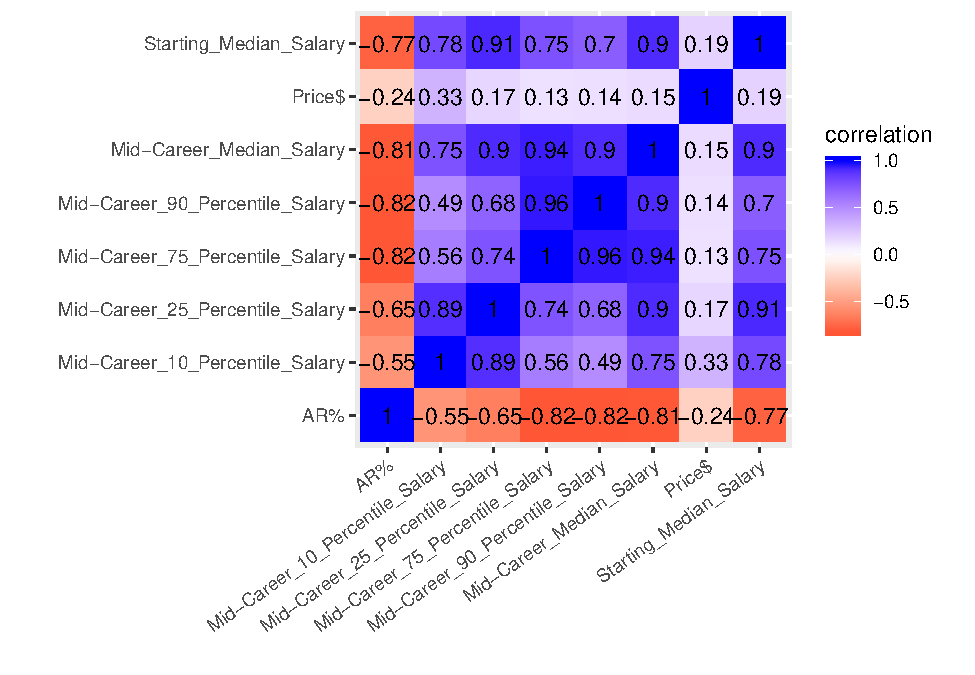
\includegraphics{project1_files/figure-latex/unnamed-chunk-4-1} \end{center}

\begin{Shaded}
\begin{Highlighting}[]
\KeywordTok{ggplot}\NormalTok{(fulldata, }\KeywordTok{aes}\NormalTok{(Starting_Median_Salary, }\StringTok{`}\DataTypeTok{Mid-Career_Median_Salary}\StringTok{`}\NormalTok{)) }\OperatorTok{+}\StringTok{ }
\StringTok{    }\KeywordTok{geom_point}\NormalTok{(}\KeywordTok{aes}\NormalTok{(}\DataTypeTok{y =} \StringTok{`}\DataTypeTok{Mid-Career_Median_Salary}\StringTok{`}\NormalTok{, }\DataTypeTok{color =}\NormalTok{ School_Type), }
        \DataTypeTok{stat =} \StringTok{"summary"}\NormalTok{, }\DataTypeTok{fun.y =} \StringTok{"mean"}\NormalTok{) }\OperatorTok{+}\StringTok{ }\KeywordTok{ggtitle}\NormalTok{(}\StringTok{"Starting Median Salary and Mid-Career Median Salary by School Type"}\NormalTok{) }\OperatorTok{+}\StringTok{ }
\StringTok{    }\KeywordTok{scale_y_continuous}\NormalTok{(}\DataTypeTok{name =} \StringTok{"Mid-Career Median Salary (USD)"}\NormalTok{) }\OperatorTok{+}\StringTok{ }
\StringTok{    }\KeywordTok{xlab}\NormalTok{(}\StringTok{"Starting Median Salary (USD)"}\NormalTok{) }\OperatorTok{+}\StringTok{ }\KeywordTok{theme_light}\NormalTok{(}\DataTypeTok{base_size =} \DecValTok{10}\NormalTok{) }\OperatorTok{+}\StringTok{ }
\StringTok{    }\KeywordTok{scale_color_brewer}\NormalTok{(}\DataTypeTok{palette =} \StringTok{"Dark2"}\NormalTok{)}
\end{Highlighting}
\end{Shaded}

\begin{center}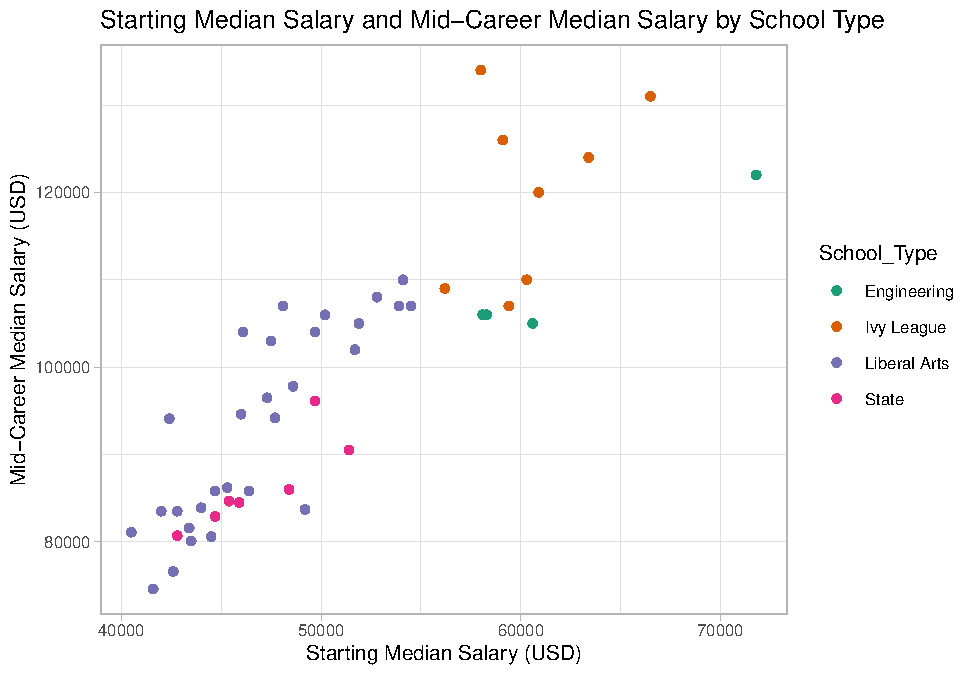
\includegraphics{project1_files/figure-latex/unnamed-chunk-4-2} \end{center}

\begin{Shaded}
\begin{Highlighting}[]
\NormalTok{newAR <-}\StringTok{ }\NormalTok{byschooltype }\OperatorTok\StringTok{ }\KeywordTok{mutate}\NormalTok{(}\DataTypeTok{AR_cat =} \KeywordTok{case_when}\NormalTok{(}\StringTok{`}\DataTypeTok{AR%}\StringTok{`} \OperatorTok{>}\StringTok{ }\DecValTok{33} \OperatorTok{~}\StringTok{ }
\StringTok{    "high"}\NormalTok{, }\StringTok{`}\DataTypeTok{AR%}\StringTok{`} \OperatorTok{==}\StringTok{ }\DecValTok{33} \OperatorTok{~}\StringTok{ "high"}\NormalTok{, }\StringTok{`}\DataTypeTok{AR%}\StringTok{`} \OperatorTok{<}\StringTok{ }\DecValTok{33} \OperatorTok{~}\StringTok{ "low"}\NormalTok{))}

\KeywordTok{ggplot}\NormalTok{(newAR, }\KeywordTok{aes}\NormalTok{(AR_cat, }\StringTok{`}\DataTypeTok{Price$}\StringTok{`}\NormalTok{)) }\OperatorTok{+}\StringTok{ }\KeywordTok{geom_bar}\NormalTok{(}\KeywordTok{aes}\NormalTok{(}\DataTypeTok{y =} \StringTok{`}\DataTypeTok{Price$}\StringTok{`}\NormalTok{, }
    \DataTypeTok{fill =}\NormalTok{ School_Type), }\DataTypeTok{stat =} \StringTok{"summary"}\NormalTok{, }\DataTypeTok{fun.y =} \StringTok{"mean"}\NormalTok{) }\OperatorTok{+}\StringTok{ }
\StringTok{    }\KeywordTok{ggtitle}\NormalTok{(}\StringTok{"Acceptance Rate and Cost of Attendance by School Type"}\NormalTok{) }\OperatorTok{+}\StringTok{ }
\StringTok{    }\KeywordTok{xlab}\NormalTok{(}\StringTok{"Acceptance Rate"}\NormalTok{) }\OperatorTok{+}\StringTok{ }\KeywordTok{ylab}\NormalTok{(}\StringTok{"Cost of Attendance (USD)"}\NormalTok{) }\OperatorTok{+}\StringTok{ }
\StringTok{    }\KeywordTok{scale_fill_brewer}\NormalTok{() }\OperatorTok{+}\StringTok{ }\KeywordTok{theme_light}\NormalTok{(}\DataTypeTok{base_size =} \DecValTok{12}\NormalTok{) }\OperatorTok{+}\StringTok{ }\KeywordTok{scale_y_continuous}\NormalTok{(}\DataTypeTok{breaks =} \KeywordTok{seq}\NormalTok{(}\DecValTok{0}\NormalTok{, }
    \DecValTok{80000}\NormalTok{, }\DecValTok{10000}\NormalTok{))}
\end{Highlighting}
\end{Shaded}

\begin{center}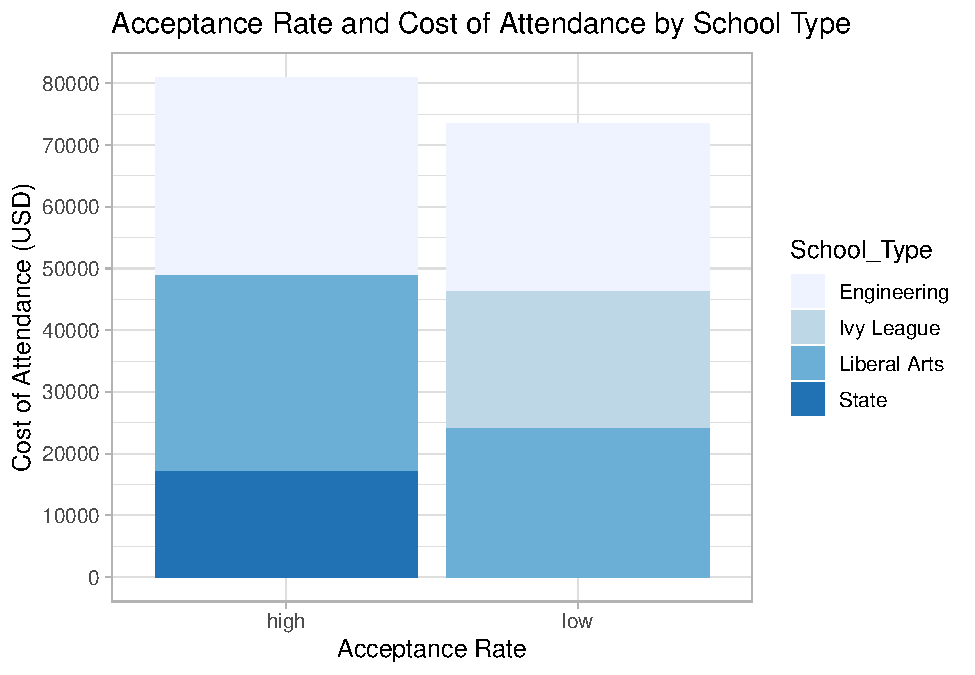
\includegraphics{project1_files/figure-latex/unnamed-chunk-4-3} \end{center}

In the correlation matrix, a correlation is given between every numeric
variable. The strongest correlation is 0.96 between mid-career 90th
percentile salary and mid-career 75th percentile salary. The weakest
correlation is 0.13 between cost of attendance and mid-career 75th
percentile salary. In the second plot, the correlation between starting
median salary and mid-career median salary by school type is explored.
As starting median salary increases, so does mid-career median salary,
suggesting that there is a strong positive correlation between these two
variables. The points are colored by school type and it is interesting
to note that Ivy Leagues and Engineering schools have the highest
salaries and Liberal Arts schools and State schools have lower salaries.
This indicates that schools that have higher starting median salaries
are also likely to have higher mid-career median salaries, although a
few Liberal Arts schools surpassed Ivy League and Engineering schools in
mid-career median salaries despite having a lower starting median
salary.

In the second plot, the relationship between accceptance rate and cost
of attendance was explored based on school type. To begin, I mutated
acceptance rate from a numeric variable to a categorical variable by
recoding all acceptance rates above the mean to ``high'', indicating
that these schools had a high acceptance rate, and recoded all
acceptance rates below or equal to the mean to ``low'', indicating that
these schools had low acceptance rates. I also changed the number of
tick marks on the y-axis to include more cost of attendance prices.
After completing these actions, I noticed a few relationships in this
plot. To begin with, no State schools were classified as having a low
acceptance rate and no Ivy Leagues were classified as having a high
acceptance rate, but the other two school types fell into both
categories. It is also interesting that State schools appear to have the
lowest cost of attendance while Engineering and Liberal Arts schools
seem to have similar cost of attendance prices. Ivy Leagues appear to
cost less than Engineering and Liberal Arts schools with low acceptance
rates, which was surprising.

\section{Dimensionality Reduction}\label{dimensionality-reduction}

\begin{Shaded}
\begin{Highlighting}[]
\KeywordTok{library}\NormalTok{(}\StringTok{"tidyverse"}\NormalTok{)}
\KeywordTok{install.packages}\NormalTok{(}\StringTok{"GGally"}\NormalTok{)}
\KeywordTok{library}\NormalTok{(}\StringTok{"GGally"}\NormalTok{)}
\KeywordTok{library}\NormalTok{(cluster)}
\KeywordTok{library}\NormalTok{(dplyr)}
\KeywordTok{library}\NormalTok{(ggplot2)}

\CommentTok{# K-means Clustering}

\NormalTok{fulldata2 <-}\StringTok{ }\NormalTok{fulldata }\OperatorTok\StringTok{ }\NormalTok{dplyr}\OperatorTok{::}\KeywordTok{select}\NormalTok{(}\OperatorTok{-}\NormalTok{Institution, }\OperatorTok{-}\NormalTok{School_Type, }
    \OperatorTok{-}\NormalTok{Location, }\OperatorTok{-}\StringTok{`}\DataTypeTok{Mid-Career_10_Percentile_Salary}\StringTok{`}\NormalTok{, }\OperatorTok{-}\StringTok{`}\DataTypeTok{Mid-Career_90_Percentile_Salary}\StringTok{`}\NormalTok{)}
\NormalTok{fulldata2}
\end{Highlighting}
\end{Shaded}

\begin{verbatim}
## # A tibble: 50 x 7
##    Starting_Median~ `Mid-Career_Med~ `Mid-Career_25_~ `Mid-Career_75_~ `AR%`
##               <dbl>            <dbl>            <dbl>            <dbl> <dbl>
##  1            71800           122000            96000           180000    15
##  2            58300           106000            85200           137000    23
##  3            58100           106000            87900           142000    56
##  4            60600           105000            81900           138000    44
##  5            54100           110000            80600           156000    31
##  6            52800           108000            76700           167000    28
##  7            54500           107000            84900           162000    13
##  8            53900           107000            79300           144000    31
##  9            48100           107000            74600           146000    14
## 10            50200           106000            65600           143000    40
## # ... with 40 more rows, and 2 more variables: `Price$` <dbl>, SAT_Range <chr>
\end{verbatim}

\begin{Shaded}
\begin{Highlighting}[]
\NormalTok{wss <-}\StringTok{ }\KeywordTok{vector}\NormalTok{()}
\ControlFlowTok{for}\NormalTok{ (i }\ControlFlowTok{in} \DecValTok{1}\OperatorTok{:}\DecValTok{10}\NormalTok{) \{}
\NormalTok{    temp <-}\StringTok{ }\NormalTok{fulldata2 }\OperatorTok\StringTok{ }\KeywordTok{select}\NormalTok{(}\StringTok{`}\DataTypeTok{AR%}\StringTok{`}\NormalTok{, }\StringTok{`}\DataTypeTok{Price$}\StringTok{`}\NormalTok{) }\OperatorTok\StringTok{ }\KeywordTok{kmeans}\NormalTok{(i)}
\NormalTok{    wss[i] <-}\StringTok{ }\NormalTok{temp}\OperatorTok{$}\NormalTok{tot.withinss}
\NormalTok{\}}
\KeywordTok{ggplot}\NormalTok{() }\OperatorTok{+}\StringTok{ }\KeywordTok{geom_point}\NormalTok{(}\KeywordTok{aes}\NormalTok{(}\DataTypeTok{x =} \DecValTok{1}\OperatorTok{:}\DecValTok{10}\NormalTok{, }\DataTypeTok{y =}\NormalTok{ wss)) }\OperatorTok{+}\StringTok{ }\KeywordTok{geom_path}\NormalTok{(}\KeywordTok{aes}\NormalTok{(}\DataTypeTok{x =} \DecValTok{1}\OperatorTok{:}\DecValTok{10}\NormalTok{, }
    \DataTypeTok{y =}\NormalTok{ wss)) }\OperatorTok{+}\StringTok{ }\KeywordTok{xlab}\NormalTok{(}\StringTok{"clusters"}\NormalTok{) }\OperatorTok{+}\StringTok{ }\KeywordTok{scale_x_continuous}\NormalTok{(}\DataTypeTok{breaks =} \DecValTok{1}\OperatorTok{:}\DecValTok{10}\NormalTok{)}
\end{Highlighting}
\end{Shaded}

\begin{center}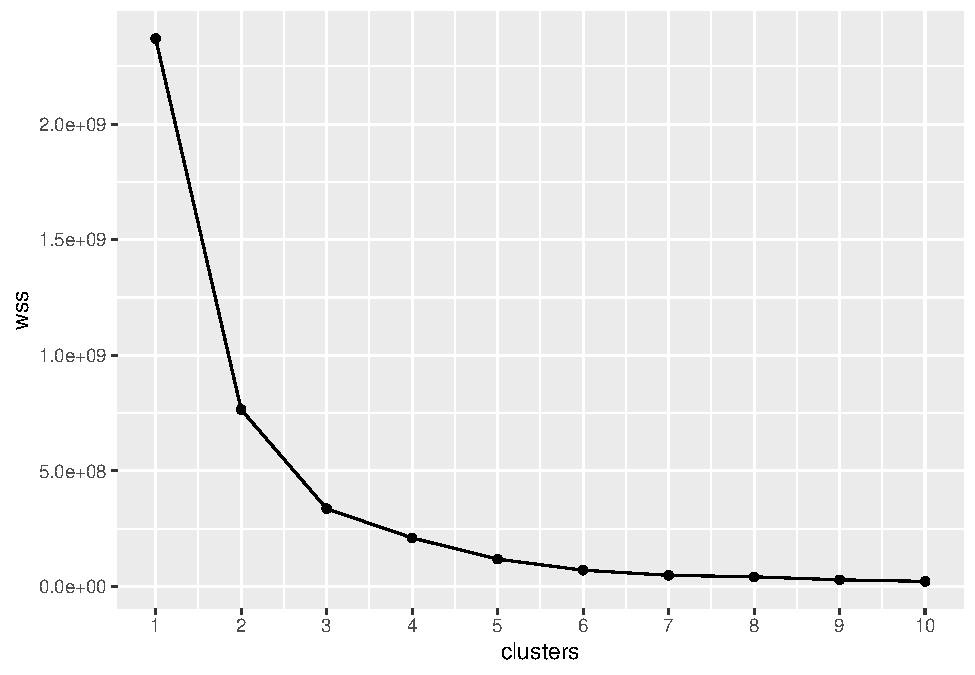
\includegraphics{project1_files/figure-latex/unnamed-chunk-5-1} \end{center}

\begin{Shaded}
\begin{Highlighting}[]
\NormalTok{cluster1 <-}\StringTok{ }\NormalTok{fulldata2 }\OperatorTok\StringTok{ }\NormalTok{dplyr}\OperatorTok{::}\KeywordTok{select}\NormalTok{(}\StringTok{`}\DataTypeTok{AR%}\StringTok{`}\NormalTok{, }\StringTok{`}\DataTypeTok{Price$}\StringTok{`}\NormalTok{)}
\NormalTok{cluster2 <-}\StringTok{ }\NormalTok{fulldata2 }\OperatorTok\StringTok{ }\NormalTok{dplyr}\OperatorTok{::}\KeywordTok{select}\NormalTok{(Starting_Median_Salary, }
    \StringTok{`}\DataTypeTok{Mid-Career_Median_Salary}\StringTok{`}\NormalTok{)}
\NormalTok{cluster3 <-}\StringTok{ }\NormalTok{fulldata2 }\OperatorTok\StringTok{ }\NormalTok{dplyr}\OperatorTok{::}\KeywordTok{select}\NormalTok{(}\StringTok{`}\DataTypeTok{Price$}\StringTok{`}\NormalTok{, }\StringTok{`}\DataTypeTok{Mid-Career_Median_Salary}\StringTok{`}\NormalTok{)}

\NormalTok{kmeans1 <-}\StringTok{ }\NormalTok{cluster1 }\OperatorTok\StringTok{ }\NormalTok{scale }\OperatorTok\StringTok{ }\KeywordTok{kmeans}\NormalTok{(}\DecValTok{2}\NormalTok{)}
\NormalTok{kmeans1}
\end{Highlighting}
\end{Shaded}

\begin{verbatim}
## K-means clustering with 2 clusters of sizes 20, 30
## 
## Cluster means:
##          AR%     Price$
## 1  0.2994486  0.9656736
## 2 -0.1996324 -0.6437824
## 
## Clustering vector:
##  [1] 1 2 1 1 1 2 2 2 2 1 1 2 1 1 2 2 2 2 2 2 1 1 2 1 1 2 2 1 1 1 1 1 1 2 2 2 2 2
## [39] 2 1 2 2 2 2 2 1 2 2 2 2
## 
## Within cluster sum of squares by cluster:
## [1] 21.31712 42.60972
##  (between_SS / total_SS =  34.8 %)
## 
## Available components:
## 
## [1] "cluster"      "centers"      "totss"        "withinss"     "tot.withinss"
## [6] "betweenss"    "size"         "iter"         "ifault"
\end{verbatim}

\begin{Shaded}
\begin{Highlighting}[]
\NormalTok{kmeans1}\OperatorTok{$}\NormalTok{size}
\end{Highlighting}
\end{Shaded}

\begin{verbatim}
## [1] 20 30
\end{verbatim}

\begin{Shaded}
\begin{Highlighting}[]
\NormalTok{kmeans1}\OperatorTok{$}\NormalTok{center}
\end{Highlighting}
\end{Shaded}

\begin{verbatim}
##          AR%     Price$
## 1  0.2994486  0.9656736
## 2 -0.1996324 -0.6437824
\end{verbatim}

\begin{Shaded}
\begin{Highlighting}[]
\NormalTok{kmeans1}\OperatorTok{$}\NormalTok{cluster}
\end{Highlighting}
\end{Shaded}

\begin{verbatim}
##  [1] 1 2 1 1 1 2 2 2 2 1 1 2 1 1 2 2 2 2 2 2 1 1 2 1 1 2 2 1 1 1 1 1 1 2 2 2 2 2
## [39] 2 1 2 2 2 2 2 1 2 2 2 2
\end{verbatim}

\begin{Shaded}
\begin{Highlighting}[]
\NormalTok{kmeansclust <-}\StringTok{ }\NormalTok{fulldata2 }\OperatorTok\StringTok{ }\KeywordTok{mutate}\NormalTok{(}\DataTypeTok{cluster =} \KeywordTok{as.factor}\NormalTok{(kmeans1}\OperatorTok{$}\NormalTok{cluster))}
\NormalTok{kmeansclust }\OperatorTok\StringTok{ }\KeywordTok{ggplot}\NormalTok{(}\KeywordTok{aes}\NormalTok{(}\StringTok{`}\DataTypeTok{AR%}\StringTok{`}\NormalTok{, }\StringTok{`}\DataTypeTok{Price$}\StringTok{`}\NormalTok{, }\DataTypeTok{color =}\NormalTok{ cluster)) }\OperatorTok{+}\StringTok{ }
\StringTok{    }\KeywordTok{geom_point}\NormalTok{()}
\end{Highlighting}
\end{Shaded}

\begin{center}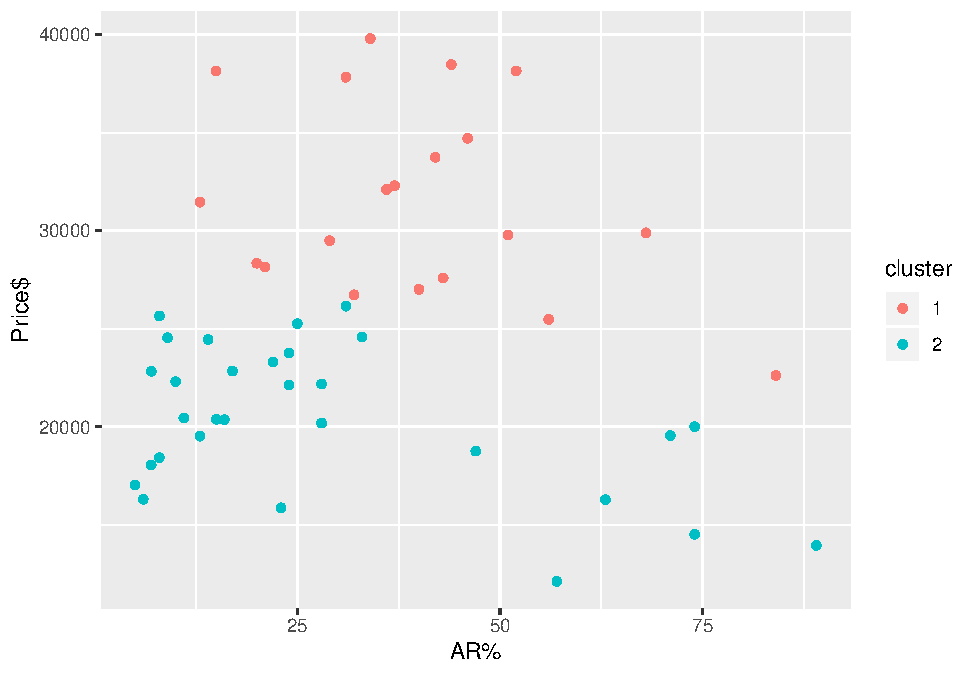
\includegraphics{project1_files/figure-latex/unnamed-chunk-5-2} \end{center}

\begin{Shaded}
\begin{Highlighting}[]
\NormalTok{wss2 <-}\StringTok{ }\KeywordTok{vector}\NormalTok{()}
\ControlFlowTok{for}\NormalTok{ (i }\ControlFlowTok{in} \DecValTok{1}\OperatorTok{:}\DecValTok{10}\NormalTok{) \{}
\NormalTok{    temp <-}\StringTok{ }\NormalTok{fulldata2 }\OperatorTok\StringTok{ }\KeywordTok{select}\NormalTok{(Starting_Median_Salary, }\StringTok{`}\DataTypeTok{Mid-Career_Median_Salary}\StringTok{`}\NormalTok{) }\OperatorTok\StringTok{ }
\StringTok{        }\KeywordTok{kmeans}\NormalTok{(i)}
\NormalTok{    wss[i] <-}\StringTok{ }\NormalTok{temp}\OperatorTok{$}\NormalTok{tot.withinss}
\NormalTok{\}}
\KeywordTok{ggplot}\NormalTok{() }\OperatorTok{+}\StringTok{ }\KeywordTok{geom_point}\NormalTok{(}\KeywordTok{aes}\NormalTok{(}\DataTypeTok{x =} \DecValTok{1}\OperatorTok{:}\DecValTok{10}\NormalTok{, }\DataTypeTok{y =}\NormalTok{ wss)) }\OperatorTok{+}\StringTok{ }\KeywordTok{geom_path}\NormalTok{(}\KeywordTok{aes}\NormalTok{(}\DataTypeTok{x =} \DecValTok{1}\OperatorTok{:}\DecValTok{10}\NormalTok{, }
    \DataTypeTok{y =}\NormalTok{ wss)) }\OperatorTok{+}\StringTok{ }\KeywordTok{xlab}\NormalTok{(}\StringTok{"clusters"}\NormalTok{) }\OperatorTok{+}\StringTok{ }\KeywordTok{scale_x_continuous}\NormalTok{(}\DataTypeTok{breaks =} \DecValTok{1}\OperatorTok{:}\DecValTok{10}\NormalTok{)}
\end{Highlighting}
\end{Shaded}

\begin{center}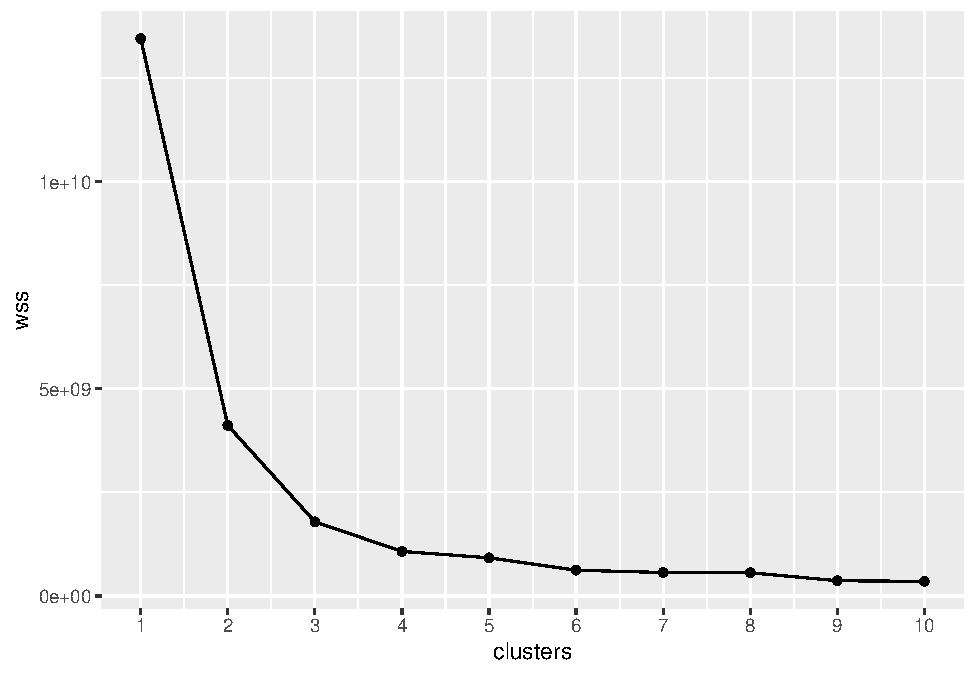
\includegraphics{project1_files/figure-latex/unnamed-chunk-5-3} \end{center}

\begin{Shaded}
\begin{Highlighting}[]
\NormalTok{kmeans2 <-}\StringTok{ }\NormalTok{cluster2 }\OperatorTok\StringTok{ }\NormalTok{scale }\OperatorTok\StringTok{ }\KeywordTok{kmeans}\NormalTok{(}\DecValTok{2}\NormalTok{)}
\NormalTok{kmeans2}
\end{Highlighting}
\end{Shaded}

\begin{verbatim}
## K-means clustering with 2 clusters of sizes 31, 19
## 
## Cluster means:
##   Starting_Median_Salary Mid-Career_Median_Salary
## 1             -0.6493326                -0.615673
## 2              1.0594375                 1.004519
## 
## Clustering vector:
##  [1] 2 2 2 2 2 2 2 2 1 2 2 1 1 1 2 1 1 1 1 1 1 1 1 1 1 1 1 1 1 1 1 1 1 1 2 2 2 2
## [39] 2 2 2 2 1 1 1 1 1 1 1 1
## 
## Within cluster sum of squares by cluster:
## [1] 14.64982 18.03105
##  (between_SS / total_SS =  66.7 %)
## 
## Available components:
## 
## [1] "cluster"      "centers"      "totss"        "withinss"     "tot.withinss"
## [6] "betweenss"    "size"         "iter"         "ifault"
\end{verbatim}

\begin{Shaded}
\begin{Highlighting}[]
\NormalTok{kmeans2}\OperatorTok{$}\NormalTok{size}
\end{Highlighting}
\end{Shaded}

\begin{verbatim}
## [1] 31 19
\end{verbatim}

\begin{Shaded}
\begin{Highlighting}[]
\NormalTok{kmeans2}\OperatorTok{$}\NormalTok{center}
\end{Highlighting}
\end{Shaded}

\begin{verbatim}
##   Starting_Median_Salary Mid-Career_Median_Salary
## 1             -0.6493326                -0.615673
## 2              1.0594375                 1.004519
\end{verbatim}

\begin{Shaded}
\begin{Highlighting}[]
\NormalTok{kmeans2}\OperatorTok{$}\NormalTok{cluster}
\end{Highlighting}
\end{Shaded}

\begin{verbatim}
##  [1] 2 2 2 2 2 2 2 2 1 2 2 1 1 1 2 1 1 1 1 1 1 1 1 1 1 1 1 1 1 1 1 1 1 1 2 2 2 2
## [39] 2 2 2 2 1 1 1 1 1 1 1 1
\end{verbatim}

\begin{Shaded}
\begin{Highlighting}[]
\NormalTok{kmeansclust2 <-}\StringTok{ }\NormalTok{fulldata2 }\OperatorTok\StringTok{ }\KeywordTok{mutate}\NormalTok{(}\DataTypeTok{cluster =} \KeywordTok{as.factor}\NormalTok{(kmeans1}\OperatorTok{$}\NormalTok{cluster))}
\NormalTok{kmeansclust2 }\OperatorTok\StringTok{ }\KeywordTok{ggplot}\NormalTok{(}\KeywordTok{aes}\NormalTok{(Starting_Median_Salary, }\StringTok{`}\DataTypeTok{Mid-Career_Median_Salary}\StringTok{`}\NormalTok{, }
    \DataTypeTok{color =}\NormalTok{ cluster)) }\OperatorTok{+}\StringTok{ }\KeywordTok{geom_point}\NormalTok{()}
\end{Highlighting}
\end{Shaded}

\begin{center}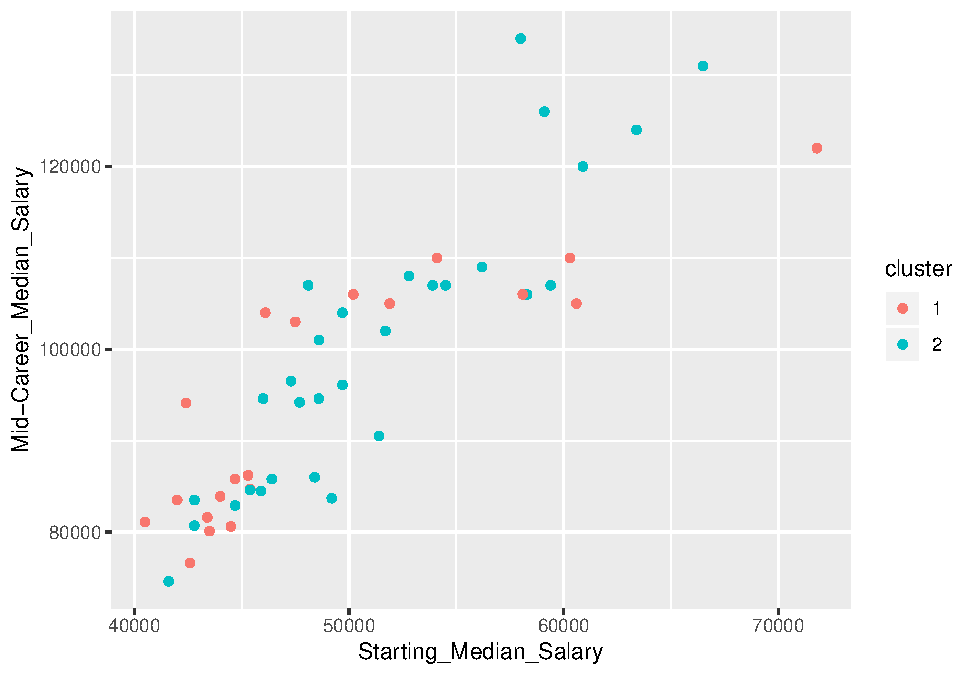
\includegraphics{project1_files/figure-latex/unnamed-chunk-5-4} \end{center}

\begin{Shaded}
\begin{Highlighting}[]
\NormalTok{wss3 <-}\StringTok{ }\KeywordTok{vector}\NormalTok{()}
\ControlFlowTok{for}\NormalTok{ (i }\ControlFlowTok{in} \DecValTok{1}\OperatorTok{:}\DecValTok{10}\NormalTok{) \{}
\NormalTok{    temp <-}\StringTok{ }\NormalTok{fulldata2 }\OperatorTok\StringTok{ }\KeywordTok{select}\NormalTok{(}\StringTok{`}\DataTypeTok{Price$}\StringTok{`}\NormalTok{, }\StringTok{`}\DataTypeTok{Mid-Career_Median_Salary}\StringTok{`}\NormalTok{) }\OperatorTok\StringTok{ }
\StringTok{        }\KeywordTok{kmeans}\NormalTok{(i)}
\NormalTok{    wss[i] <-}\StringTok{ }\NormalTok{temp}\OperatorTok{$}\NormalTok{tot.withinss}
\NormalTok{\}}
\KeywordTok{ggplot}\NormalTok{() }\OperatorTok{+}\StringTok{ }\KeywordTok{geom_point}\NormalTok{(}\KeywordTok{aes}\NormalTok{(}\DataTypeTok{x =} \DecValTok{1}\OperatorTok{:}\DecValTok{10}\NormalTok{, }\DataTypeTok{y =}\NormalTok{ wss)) }\OperatorTok{+}\StringTok{ }\KeywordTok{geom_path}\NormalTok{(}\KeywordTok{aes}\NormalTok{(}\DataTypeTok{x =} \DecValTok{1}\OperatorTok{:}\DecValTok{10}\NormalTok{, }
    \DataTypeTok{y =}\NormalTok{ wss)) }\OperatorTok{+}\StringTok{ }\KeywordTok{xlab}\NormalTok{(}\StringTok{"clusters"}\NormalTok{) }\OperatorTok{+}\StringTok{ }\KeywordTok{scale_x_continuous}\NormalTok{(}\DataTypeTok{breaks =} \DecValTok{1}\OperatorTok{:}\DecValTok{10}\NormalTok{)}
\end{Highlighting}
\end{Shaded}

\begin{center}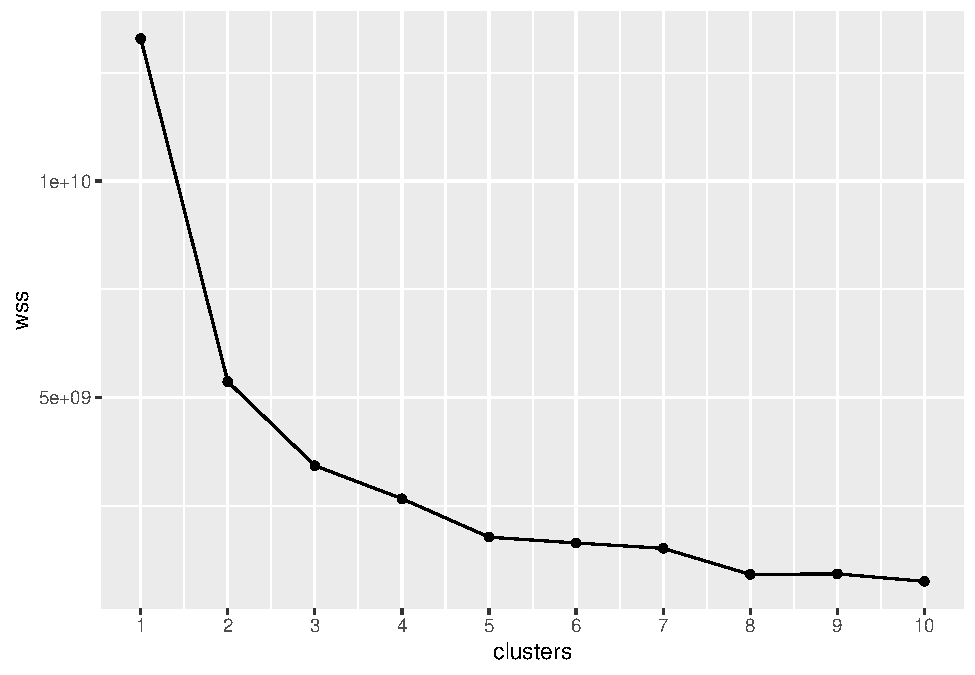
\includegraphics{project1_files/figure-latex/unnamed-chunk-5-5} \end{center}

\begin{Shaded}
\begin{Highlighting}[]
\NormalTok{kmeans3 <-}\StringTok{ }\NormalTok{cluster3 }\OperatorTok\StringTok{ }\NormalTok{scale }\OperatorTok\StringTok{ }\KeywordTok{kmeans}\NormalTok{(}\DecValTok{2}\NormalTok{)}
\NormalTok{kmeans3}
\end{Highlighting}
\end{Shaded}

\begin{verbatim}
## K-means clustering with 2 clusters of sizes 32, 18
## 
## Cluster means:
##       Price$ Mid-Career_Median_Salary
## 1 -0.6031041                0.1990902
## 2  1.0721850               -0.3539381
## 
## Clustering vector:
##  [1] 2 1 1 2 2 1 1 1 1 1 2 1 2 2 1 1 1 1 1 1 2 2 1 2 2 1 1 2 2 2 2 2 2 2 1 1 1 1
## [39] 1 2 1 1 1 1 1 1 1 1 1 1
## 
## Within cluster sum of squares by cluster:
## [1] 39.51511 22.62965
##  (between_SS / total_SS =  36.6 %)
## 
## Available components:
## 
## [1] "cluster"      "centers"      "totss"        "withinss"     "tot.withinss"
## [6] "betweenss"    "size"         "iter"         "ifault"
\end{verbatim}

\begin{Shaded}
\begin{Highlighting}[]
\NormalTok{kmeans3}\OperatorTok{$}\NormalTok{size}
\end{Highlighting}
\end{Shaded}

\begin{verbatim}
## [1] 32 18
\end{verbatim}

\begin{Shaded}
\begin{Highlighting}[]
\NormalTok{kmeans3}\OperatorTok{$}\NormalTok{center}
\end{Highlighting}
\end{Shaded}

\begin{verbatim}
##       Price$ Mid-Career_Median_Salary
## 1 -0.6031041                0.1990902
## 2  1.0721850               -0.3539381
\end{verbatim}

\begin{Shaded}
\begin{Highlighting}[]
\NormalTok{kmeans3}\OperatorTok{$}\NormalTok{cluster}
\end{Highlighting}
\end{Shaded}

\begin{verbatim}
##  [1] 2 1 1 2 2 1 1 1 1 1 2 1 2 2 1 1 1 1 1 1 2 2 1 2 2 1 1 2 2 2 2 2 2 2 1 1 1 1
## [39] 1 2 1 1 1 1 1 1 1 1 1 1
\end{verbatim}

\begin{Shaded}
\begin{Highlighting}[]
\NormalTok{kmeansclust3 <-}\StringTok{ }\NormalTok{fulldata2 }\OperatorTok\StringTok{ }\KeywordTok{mutate}\NormalTok{(}\DataTypeTok{cluster =} \KeywordTok{as.factor}\NormalTok{(kmeans1}\OperatorTok{$}\NormalTok{cluster))}
\NormalTok{kmeansclust3 }\OperatorTok\StringTok{ }\KeywordTok{ggplot}\NormalTok{(}\KeywordTok{aes}\NormalTok{(}\StringTok{`}\DataTypeTok{Price$}\StringTok{`}\NormalTok{, }\StringTok{`}\DataTypeTok{Mid-Career_Median_Salary}\StringTok{`}\NormalTok{, }
    \DataTypeTok{color =}\NormalTok{ cluster)) }\OperatorTok{+}\StringTok{ }\KeywordTok{geom_point}\NormalTok{()}
\end{Highlighting}
\end{Shaded}

\begin{center}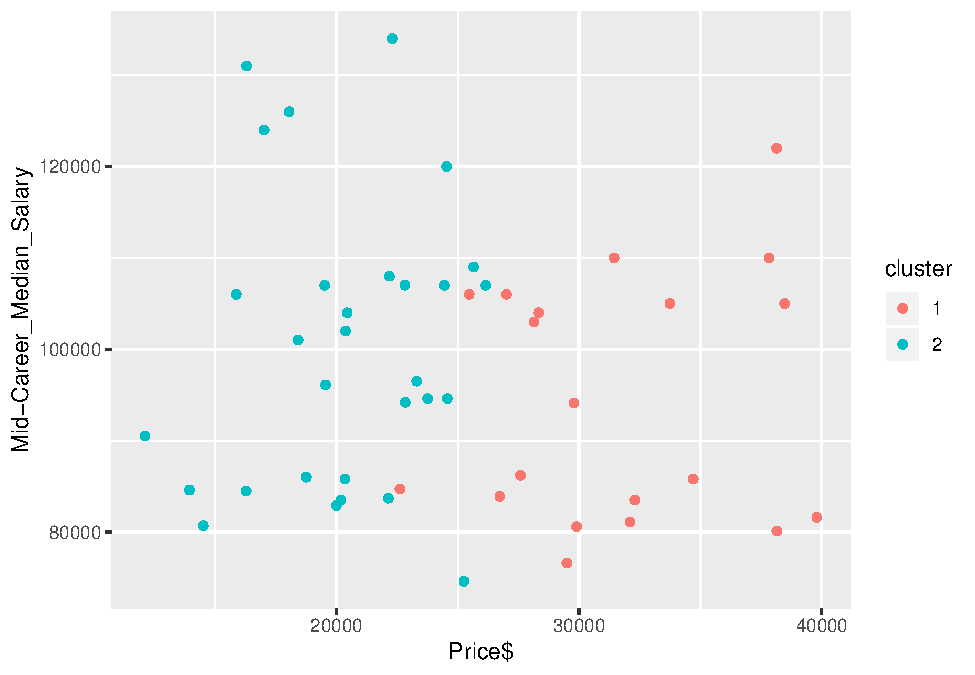
\includegraphics{project1_files/figure-latex/unnamed-chunk-5-6} \end{center}

\begin{Shaded}
\begin{Highlighting}[]
\CommentTok{# PAM}
\NormalTok{pam_dat <-}\StringTok{ }\NormalTok{fulldata2 }\OperatorTok\StringTok{ }\KeywordTok{select}\NormalTok{(}\StringTok{`}\DataTypeTok{AR%}\StringTok{`}\NormalTok{, }\StringTok{`}\DataTypeTok{Price$}\StringTok{`}\NormalTok{)}
\NormalTok{sil_width <-}\StringTok{ }\KeywordTok{vector}\NormalTok{()}
\ControlFlowTok{for}\NormalTok{ (i }\ControlFlowTok{in} \DecValTok{2}\OperatorTok{:}\DecValTok{10}\NormalTok{) \{}
\NormalTok{    pam_fit <-}\StringTok{ }\KeywordTok{pam}\NormalTok{(pam_dat, }\DataTypeTok{k =}\NormalTok{ i)}
\NormalTok{    sil_width[i] <-}\StringTok{ }\NormalTok{pam_fit}\OperatorTok{$}\NormalTok{silinfo}\OperatorTok{$}\NormalTok{avg.width}
\NormalTok{\}}
\KeywordTok{ggplot}\NormalTok{() }\OperatorTok{+}\StringTok{ }\KeywordTok{geom_line}\NormalTok{(}\KeywordTok{aes}\NormalTok{(}\DataTypeTok{x =} \DecValTok{1}\OperatorTok{:}\DecValTok{10}\NormalTok{, }\DataTypeTok{y =}\NormalTok{ sil_width)) }\OperatorTok{+}\StringTok{ }\KeywordTok{scale_x_continuous}\NormalTok{(}\DataTypeTok{name =} \StringTok{"k"}\NormalTok{, }
    \DataTypeTok{breaks =} \DecValTok{1}\OperatorTok{:}\DecValTok{10}\NormalTok{)}
\end{Highlighting}
\end{Shaded}

\begin{center}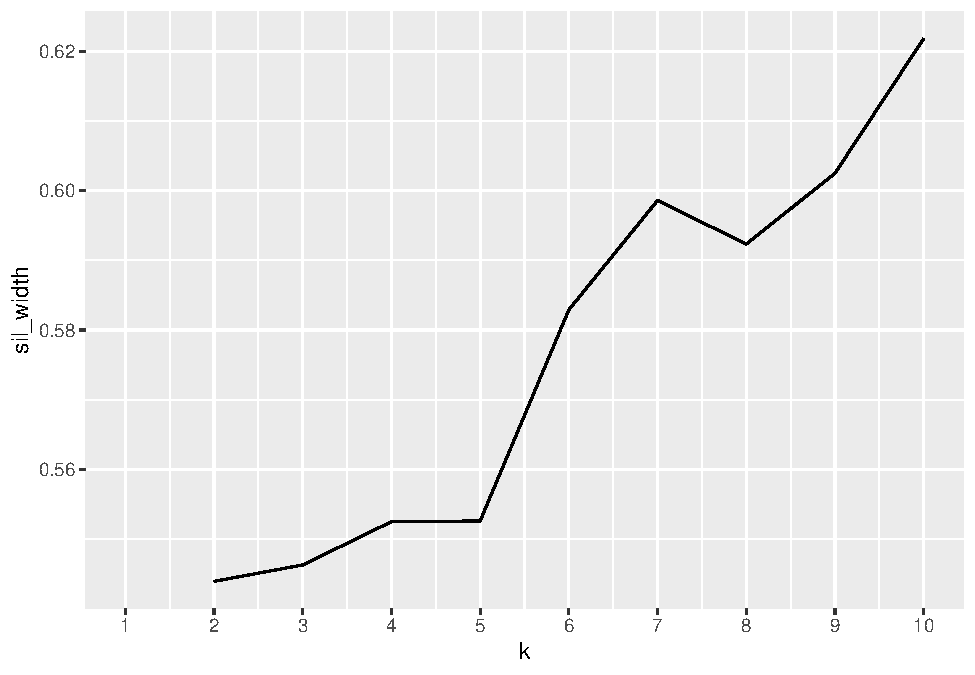
\includegraphics{project1_files/figure-latex/unnamed-chunk-5-7} \end{center}

\begin{Shaded}
\begin{Highlighting}[]
\NormalTok{pam1 <-}\StringTok{ }\NormalTok{fulldata2 }\OperatorTok\StringTok{ }\KeywordTok{pam}\NormalTok{(}\DataTypeTok{k =} \DecValTok{2}\NormalTok{)}
\NormalTok{pam1}
\end{Highlighting}
\end{Shaded}

\begin{verbatim}
## Medoids:
##      ID Starting_Median_Salary Mid-Career_Median_Salary
## [1,] 41                  56200                   109000
## [2,] 22                  45300                    86200
##      Mid-Career_25_Percentile_Salary Mid-Career_75_Percentile_Salary AR% Price$
## [1,]                           74400                          159000   8  25651
## [2,]                           61000                          120000  43  27587
##      SAT_Range
## [1,]        NA
## [2,]        NA
## Clustering vector:
##  [1] 1 1 1 1 1 1 1 1 1 1 1 1 1 1 1 1 1 1 2 2 2 2 2 2 2 2 2 2 2 2 2 2 2 2 1 1 1 1
## [39] 1 1 1 1 2 2 2 2 2 2 2 2
## Objective function:
##    build     swap 
## 24265.74 20807.94 
## 
## Available components:
##  [1] "medoids"    "id.med"     "clustering" "objective"  "isolation" 
##  [6] "clusinfo"   "silinfo"    "diss"       "call"       "data"
\end{verbatim}

\begin{Shaded}
\begin{Highlighting}[]
\NormalTok{fulldata }\OperatorTok\StringTok{ }\KeywordTok{mutate}\NormalTok{(}\DataTypeTok{cluster =} \KeywordTok{as.factor}\NormalTok{(pam1}\OperatorTok{$}\NormalTok{clustering)) }\OperatorTok\StringTok{ }
\StringTok{    }\KeywordTok{ggpairs}\NormalTok{(}\DataTypeTok{columns =} \DecValTok{2}\OperatorTok{:}\DecValTok{6}\NormalTok{, }\KeywordTok{aes}\NormalTok{(}\DataTypeTok{color =}\NormalTok{ cluster))}
\end{Highlighting}
\end{Shaded}

\begin{center}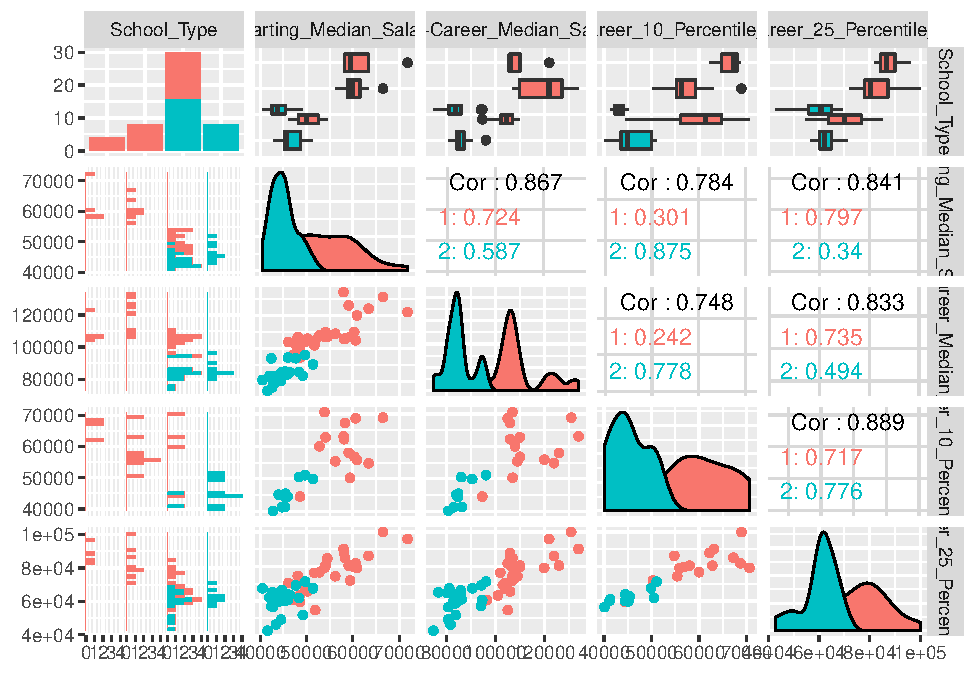
\includegraphics{project1_files/figure-latex/unnamed-chunk-5-8} \end{center}

\begin{Shaded}
\begin{Highlighting}[]
\KeywordTok{plot}\NormalTok{(pam1, }\DataTypeTok{which =} \DecValTok{2}\NormalTok{)}
\end{Highlighting}
\end{Shaded}

\begin{center}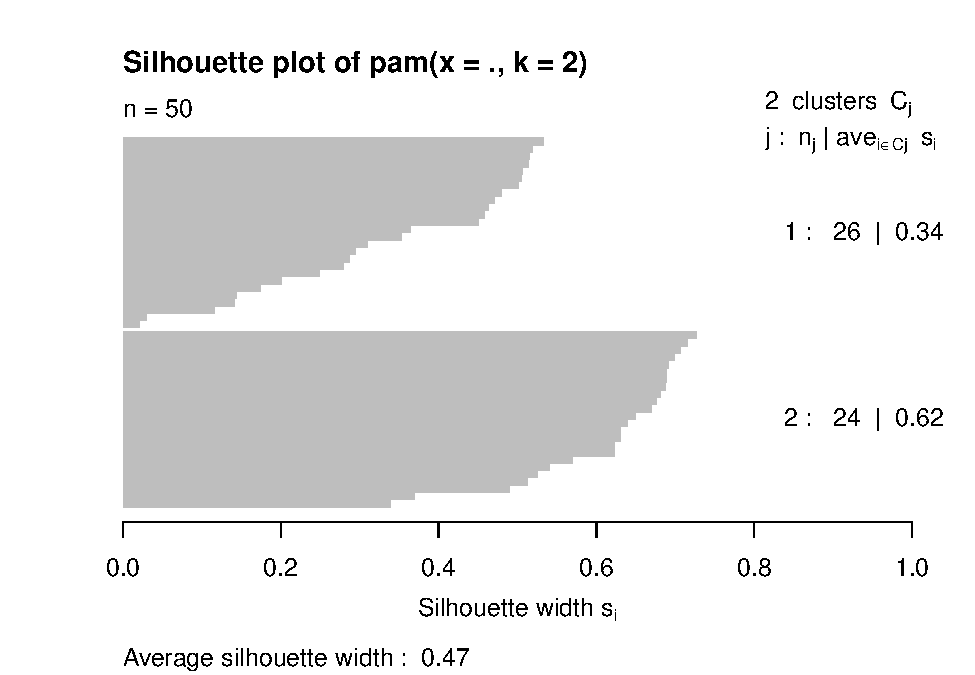
\includegraphics{project1_files/figure-latex/unnamed-chunk-5-9} \end{center}

\begin{Shaded}
\begin{Highlighting}[]
\NormalTok{pamclust <-}\StringTok{ }\NormalTok{fulldata2 }\OperatorTok\StringTok{ }\KeywordTok{mutate}\NormalTok{(}\DataTypeTok{cluster =} \KeywordTok{as.factor}\NormalTok{(pam1}\OperatorTok{$}\NormalTok{clustering))}
\NormalTok{pamclust }\OperatorTok\StringTok{ }\KeywordTok{ggplot}\NormalTok{(}\KeywordTok{aes}\NormalTok{(}\StringTok{`}\DataTypeTok{AR%}\StringTok{`}\NormalTok{, }\StringTok{`}\DataTypeTok{Price$}\StringTok{`}\NormalTok{, }\DataTypeTok{color =}\NormalTok{ cluster)) }\OperatorTok{+}\StringTok{ }
\StringTok{    }\KeywordTok{geom_point}\NormalTok{()}
\end{Highlighting}
\end{Shaded}

\begin{center}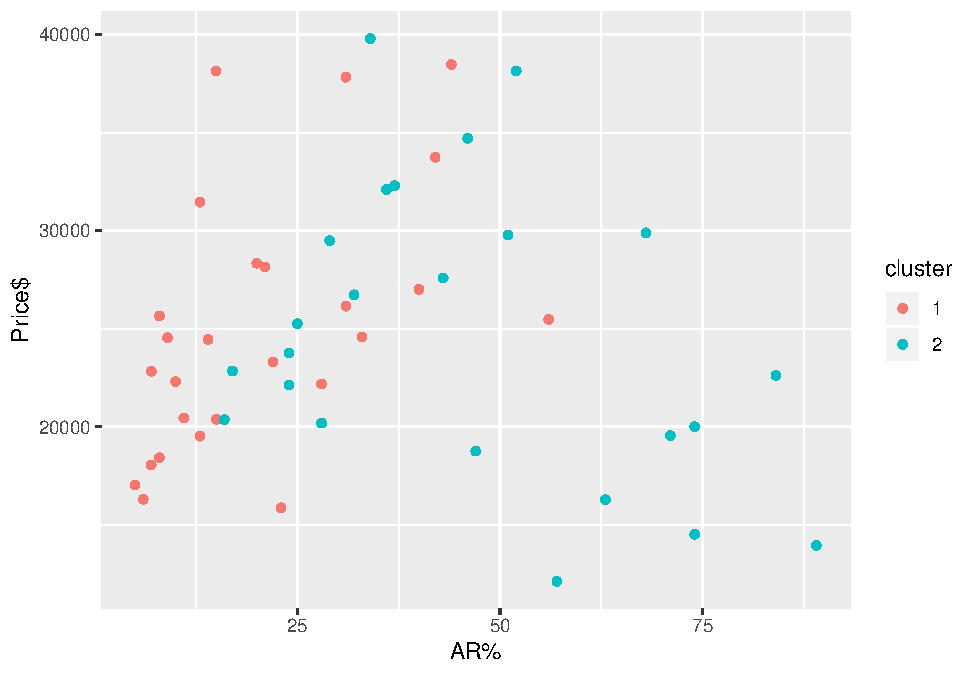
\includegraphics{project1_files/figure-latex/unnamed-chunk-5-10} \end{center}

\begin{Shaded}
\begin{Highlighting}[]
\NormalTok{pamclust }\OperatorTok\StringTok{ }\KeywordTok{group_by}\NormalTok{(cluster) }\OperatorTok\StringTok{ }\KeywordTok{summarize_if}\NormalTok{(is.numeric, mean, }
    \DataTypeTok{na.rm =}\NormalTok{ T)}
\end{Highlighting}
\end{Shaded}

\begin{verbatim}
## # A tibble: 2 x 7
##   cluster Starting_Median~ `Mid-Career_Med~ `Mid-Career_25_~ `Mid-Career_75_~
##   <fct>              <dbl>            <dbl>            <dbl>            <dbl>
## 1 1                 55292.          109812.           76796.          162154.
## 2 2                 45012.           84996.           60408.          120625 
## # ... with 2 more variables: `AR%` <dbl>, `Price$` <dbl>
\end{verbatim}

\begin{Shaded}
\begin{Highlighting}[]
\NormalTok{fulldata[pam1}\OperatorTok{$}\NormalTok{id.med, ]}
\end{Highlighting}
\end{Shaded}

\begin{verbatim}
## # A tibble: 2 x 12
##   Institution School_Type Starting_Median~ `Mid-Career_Med~ `Mid-Career_10_~
##   <chr>       <chr>                  <dbl>            <dbl>            <dbl>
## 1 Brown Univ~ Ivy League             56200           109000            55400
## 2 St. Olaf C~ Liberal Ar~            45300            86200            41300
## # ... with 7 more variables: `Mid-Career_25_Percentile_Salary` <dbl>,
## #   `Mid-Career_75_Percentile_Salary` <dbl>,
## #   `Mid-Career_90_Percentile_Salary` <dbl>, `AR%` <dbl>, Location <chr>,
## #   `Price$` <dbl>, SAT_Range <chr>
\end{verbatim}

\begin{Shaded}
\begin{Highlighting}[]
\NormalTok{pam1}\OperatorTok{$}\NormalTok{silinfo}\OperatorTok{$}\NormalTok{avg.width}
\end{Highlighting}
\end{Shaded}

\begin{verbatim}
## [1] 0.4731273
\end{verbatim}

For this dataset, I performed k-means clustering on my numeric
variables. To begin, I created new data where I removed all of the
categorical variables and then I plotted WSS against the number of
clusters to determine the best number of clusters to use. The WSS
appeared to drop rapidly at 2, and so I decided that 2 clusters was best
based on the plot. Next, I made my k-means clusters. The first k-means
cluster included the variables of acceptance rate and cost of
attendance. I scaled these variables and checked the k-means size,
center, and cluster. After assigning each of the observations to the
cluster whose center is closest and saving the cluster assignment as a
column in the dataset, I graphed this first k-means and colored the data
by final cluster assignment. I saw two distinct groups. The first
cluster has an overall lower cost of attendance than the second cluster,
however both clusters vary in acceptance rate. There does seem to be a
general trend, however, that the lower the acceptance rate the higher
cost of attendance. The size of the clusters was 30 and 20, with the
lower cost of attendance cluster having 30 institutions and the higher
cost of attendance cluster having 20 institutions.

Next, I performed a second k-means clustering on the numeric variables
of starting median salary and mid-career median salary. I first
determined how many clusters were appropriate. I decided to use 2
clusters, with one cluster having 19 institutions and the other cluster
having 32 institutions. I then created a ggplot to visualize the
clusters. These clusters appeared to be entertwined. These clusters did
not map nicely at all to these variables and there is no distinction
between the two clusters since they have similar starting median
salaries and mid-career median salaries. There is a positive correlation
between the two variables, however, in both clusters.

Finally, I performed a third k-means clustering on the numeric variables
of cost of attendance and mid-career median salary. I determined how
many clusters were appropriate for these numeric variables and once
again decided on two clusters. I graphed these clusters via ggplot. The
sizes of these clusters are 24 and 26. These clusters are separated once
again based on cost of attendance. One cluster has a consistently higher
cost of attendance while the other cluster has a consistently lower cost
of attendance, however the distinction between mid-career median salary
is not as clear. It is clear that the first and third k-means mapped
much more nicely and showed the clusters much more distinctly than the
second k-means plot. For the PAM method, I chose the number of clusters
based on average silhouette width and erred on the side of fewer
clusters. I chose 2 clusters to maximize the silhouette width. Again, I
assigned observations to the cluster whose center is closest. I saved
the cluster assignment and plotted it. I ran PAM and visualized it.
Based on this, the mid-career 10th percentile salary and mid-career 25th
percentile salary have the strongest correlation. Every correlation is
positive. In terms of the average silhouette width, which is 0.43, the
structure is considered weak and could be artifical. Next, I found the
means for each variable and the final medoids, who were most
representative of the cluster. Overall, I processed the data, chose the
number of clusters, ran both k-means and PAM cluster analysis, and
visualized the clusters. The PAM cluster did not map very nicely to the
variables or show the clusters very distinctly. Likewise, the cluster
solution was not very good, so I liked the k-means clustering plots
better and was able to interpret them better.

\begin{verbatim}
## R version 3.4.4 (2018-03-15)
## Platform: x86_64-pc-linux-gnu (64-bit)
## Running under: Ubuntu 18.04.4 LTS
## 
## Matrix products: default
## BLAS: /usr/lib/x86_64-linux-gnu/openblas/libblas.so.3
## LAPACK: /usr/lib/x86_64-linux-gnu/libopenblasp-r0.2.20.so
## 
## locale:
##  [1] LC_CTYPE=en_US.UTF-8       LC_NUMERIC=C              
##  [3] LC_TIME=en_US.UTF-8        LC_COLLATE=en_US.UTF-8    
##  [5] LC_MONETARY=en_US.UTF-8    LC_MESSAGES=en_US.UTF-8   
##  [7] LC_PAPER=en_US.UTF-8       LC_NAME=C                 
##  [9] LC_ADDRESS=C               LC_TELEPHONE=C            
## [11] LC_MEASUREMENT=en_US.UTF-8 LC_IDENTIFICATION=C       
## 
## attached base packages:
## [1] stats     graphics  grDevices utils     datasets  methods   base     
## 
## other attached packages:
##  [1] cluster_2.0.6    GGally_1.5.0     kableExtra_1.1.0 knitr_1.28      
##  [5] forcats_0.4.0    stringr_1.4.0    dplyr_0.8.3      purrr_0.3.3     
##  [9] readr_1.3.1      tidyr_1.0.0.9000 tibble_2.1.3     ggplot2_3.2.1   
## [13] tidyverse_1.3.0 
## 
## loaded via a namespace (and not attached):
##  [1] tidyselect_0.2.5   xfun_0.13          reshape2_1.4.3     haven_2.2.0       
##  [5] lattice_0.20-35    colorspace_1.4-1   vctrs_0.2.1        generics_0.0.2    
##  [9] viridisLite_0.3.0  htmltools_0.3.6    yaml_2.2.0         utf8_1.1.4        
## [13] rlang_0.4.2        pillar_1.4.2       glue_1.3.1         withr_2.1.2       
## [17] DBI_1.0.0          RColorBrewer_1.1-2 dbplyr_1.4.2       modelr_0.1.5      
## [21] readxl_1.3.1       plyr_1.8.4         lifecycle_0.1.0    munsell_0.5.0     
## [25] gtable_0.3.0       cellranger_1.1.0   rvest_0.3.5        evaluate_0.14     
## [29] labeling_0.3       fansi_0.4.0        broom_0.5.2        Rcpp_1.0.2        
## [33] scales_1.0.0       backports_1.1.4    formatR_1.7        webshot_0.5.2     
## [37] jsonlite_1.6       fs_1.3.1           hms_0.5.3          digest_0.6.20     
## [41] stringi_1.4.3      grid_3.4.4         cli_1.1.0          tools_3.4.4       
## [45] magrittr_1.5       lazyeval_0.2.2     crayon_1.3.4       pkgconfig_2.0.2   
## [49] zeallot_0.1.0      xml2_1.2.2         reprex_0.3.0       lubridate_1.7.4   
## [53] reshape_0.8.8      assertthat_0.2.1   rmarkdown_2.1      httr_1.4.1        
## [57] rstudioapi_0.10    R6_2.4.0           nlme_3.1-131       compiler_3.4.4
\end{verbatim}

\begin{verbatim}
## [1] "2020-05-08 01:03:19 CDT"
\end{verbatim}

\begin{verbatim}
##                                        sysname 
##                                        "Linux" 
##                                        release 
##                            "4.15.0-99-generic" 
##                                        version 
## "#100-Ubuntu SMP Wed Apr 22 20:32:56 UTC 2020" 
##                                       nodename 
##                   "educcomp01.ccbb.utexas.edu" 
##                                        machine 
##                                       "x86_64" 
##                                          login 
##                                      "unknown" 
##                                           user 
##                                       "smo884" 
##                                 effective_user 
##                                       "smo884"
\end{verbatim}

\end{document}
